\documentclass[11pt,fleqn]{article}
\usepackage[margin=1in,top=1in,bottom=1in]{geometry}
\usepackage{tikz}
\usepackage{mathtools}
\usepackage{longtable}
\usepackage{enumitem}
\usepackage{hyperref}
%\usepackage[dvips]{graphics}
%\usepackage[table]{xcolor}
%\usepackage{amssymb}
\usepackage{float}
%\usepackage{subfig}
\usepackage{booktabs}
\usepackage{subcaption}

\usepackage[normalem]{ulem}

\usepackage{multicol}
\usepackage{txfonts}
\usepackage{amsfonts}
\usepackage{natbib}
\usepackage{gb4e}
\usepackage[all]{xy}
\usepackage{rotating}
\usepackage{tipa}
\usepackage{multirow}
\usepackage{authblk}
\usepackage{url}
\usepackage{pdflscape}
\usepackage{rotating}
\usepackage{adjustbox}
\usepackage{array}

\def\bad{{\leavevmode\llap{*}}}
\def\marginal{{\leavevmode\llap{?}}}
\def\verymarginal{{\leavevmode\llap{??}}}
\def\swmarginal{{\leavevmode\llap{4}}}
\def\infelic{{\leavevmode\llap{\#}}}

\definecolor{airforceblue}{rgb}{0.36, 0.54, 0.66}
%\definecolor{gray}{rgb}{0.36, 0.54, 0.66}

\newcommand{\dashrule}[1][black]{%
  \color{#1}\rule[\dimexpr.5ex-.2pt]{4pt}{.4pt}\xleaders\hbox{\rule{4pt}{0pt}\rule[\dimexpr.5ex-.2pt]{4pt}{.4pt}}\hfill\kern0pt%
}

\setlength{\parindent}{.3in}
\setlength{\parskip}{0ex}

\newcommand{\yi}{\'{\symbol{16}}}
\newcommand{\nasi}{\~{\symbol{16}}}
\newcommand{\hina}{h\nasi na}
\newcommand{\ina}{\nasi na}

\newcommand{\foc}{$_{\mbox{\small F}}$}

\hyphenation{par-ti-ci-pa-tion}

\setlength{\bibhang}{0.5in}
\setlength{\bibsep}{0mm}
\bibpunct[:]{(}{)}{,}{a}{}{,}

\newcommand{\6}{\mbox{$[\hspace*{-.6mm}[$}} 
\newcommand{\9}{\mbox{$]\hspace*{-.6mm}]$}}
\newcommand{\sem}[2]{\6#1\9$^{#2}$}
\renewcommand{\ni}{\~{\i}}

\newcommand{\citepos}[1]{\citeauthor{#1}'s \citeyear{#1}}
\newcommand{\citeposs}[1]{\citeauthor{#1}'s}
\newcommand{\citetpos}[1]{\citeauthor{#1}'s (\citeyear{#1})}

\newcolumntype{R}[2]{%
    >{\adjustbox{angle=#1,lap=\width-(#2)}\bgroup}%
    l%
    <{\egroup}%
}
\newcommand*\rot{\multicolumn{1}{R{90}{0em}}}% no optional argument here, please!


\title{Which predicates are factive? An empirical investigation%
\thanks{Acknowledgments removed for review process}}

%\thanks{For helpful comments on the research presented here, we thank David Beaver, Cleo Condoravdi, Kai von Fintel, Lauri Karttunen, Mandy Simons, Greg Scontras, the anonymous reviewers for {\em Semantics and Linguistic Theory} 2018, as well as the audiences at the MIT Linguistics colloquium, the 2018 Annual Meeting of XPRAG.de and at the University of T\"ubingen. We gratefully acknowledge financial support for this research from {\em National Science Foundation} grant BCS-1452674 (JT) and the Targeted Investment for Excellence Initiative at The Ohio State University (JT).}}

\author{Author(s)}

%\author[$\circ$]{Judith Tonhauser}
%\author[$\bullet$]{Judith Degen}

%\affil[$\circ$]{The Ohio State University / University of Stuttgart}
%\affil[$\bullet$]{Stanford University}

%\renewcommand\Authands{ and }

\newcommand{\jt}[1]{\textbf{\color{blue}JT: #1}}

\begin{document}

%\tableofcontents
%\newpage

\maketitle


\begin{abstract}

It has long been assumed that properties of the content of the clausal complement distinguish factive predicates like {\em know} from non-factive predicates like {\em think}. There is, however, disagreement about which properties define factive predicates and whether the content of the complement of particular predicates exhibits the properties attributed to factive predicates. The resulting disagreement about which predicates are factive is vexatious, given the central role that the distinction between factive and non-factive predicates has played in semantic and pragmatic theorizing, especially in the study of presuppositions. This paper investigates properties of the content of the complement of clause-embedding predicates, with the goal of understanding how such predicates can be classified. We argue that factive predicates are more heterogeneous than previously assumed and that there is little empirical support for the assumed categorical distinction between factive and non-factive predicates. We conclude by discussing the implications of our findings for analyses of presuppositions and other projective content.


\end{abstract}

			
\section{Introduction}\label{s1}

A long-standing and widely held assumption is that factive predicates like {\em know} differ from non-factive predicates like {\em think} in properties of the content of the clausal complement.\footnote{But also syntax: \citealt{kiparsky-kiparsky70}, purdue MA thesis, aaron white work rochester. We ignore syntax here because it's not clear how the semantic/pragmatic properties map onto the syntactic ones, as already suggested in kk and white.} There is, however, disagreement in the literature about which properties define factive predicates and whether the content of the complement of particular predicates exhibits the properties attributed to factive predicates. As a consequence, there is disagreement about which predicates are factive. 

Consider first the defining properties of a factive predicate. In \citealt{kiparsky-kiparsky70}, the content of the complement of a factive predicate was taken to be presupposed, i.e., ``the speaker presupposes that the embedded sentence expresses a true proposition'' (p.147), in contrast to that of a non-factive predicate.\footnote{They say sentences presuppose but also talk about speakers presupposing. NEED TO ADDRESS THIS.} Diagnostic for whether the content of the complement was presupposed was projection of the content from under negation or out of a polar question (p.150f): {\em regret}, for instance, was taken to be a factive predicate because (\ref{kip}a) ``presupposes...that the door is closed'' (p.150),  whereas {\em think} was taken to be a non-factive predicate because the content of the complement does not project over negation in (\ref{kip}b). 

\begin{exe}
\ex\label{kip}
\begin{xlist}
\ex John doesn't regret that the door is closed. \hfill (\citealt[150]{kiparsky-kiparsky70})
\ex John doesn't think that the door is closed.
\end{xlist}
\end{exe}

More recently, researchers have assumed that the content of the complement of a factive predicate is not merely presupposed but also entailed (e.g., \citealt[119-123]{gazdar79a}, \citealt[355]{ccmg90}, \citealt[345]{vds92},  \citealt[3]{abbott06}, \citealt[139]{schlenker10}, \citealt[77]{anand-hacquard2014}, \citealt[fn.7]{spector-egre2015}). \citet[66f.]{beaver01}, for instance, notes that \citet[119-123]{gazdar79a} ``describes the inferences associated with factive verbs...as being indefeasible in simple affirmative sentences'', i.e., ``entailments''. \citet[355]{ccmg90} illustrate with {\em realize} that ``[a] sentence can both entail and presuppose another sentence'': {\em Joan realizes that syntax deals with sentence structure} ``both entails and presupposes'' that syntax deals with sentence structure. And \citet[139]{schlenker10}, in discussing contents of clausal complements, points to ``the pattern of inference which is characteristic of presuppositions: an entailment of the positive sentence is preserved under negation and in questions''. 

This characterization of the properties of a factive predicate differs from that assumed in \citealt{kiparsky-kiparsky70}: it requires the content of the complement to be true in all worlds in which the affirmative sentence with the clause-embedding predicate is true rather than merely requiring a speaker who utters an affirmative sentence with the predicate to presuppose the truth of the content of the complement. A predicate on which the two definitions come apart is {\em take into account}. \citet{kiparsky-kiparsky70} considered it a factive predicate because utterances by Rahim of the polar question in (\ref{kip2}a) and the affirmative sentence in (\ref{kip2}b) lead listeners to take Rahim to presuppose the truth of the content of the complement, that the groom is unreliable. But true affirmative sentences with {\em take into account} do not entail the content of the complement, as shown by the acceptability of (\ref{kip2}c).

\begin{exe}
\ex\label{kip2}
\begin{xlist}
\ex Rahim: {\em ``Did Joan take into account that the groom is unreliable?''}

\ex Rahim: {\em ``Joan took into account that the groom is unreliable.''} 

\ex Rahim said that Joan took into account that the groom is unreliable, but she was wrong to do so because the groom is a very reliable person.
\end{xlist}
\end{exe}
%On another note: The predicates identified as factive in K\&K 1970 clearly do not all entail their complements (e.g. take into account, bear in mind, make clear). 

{\em remember} is not a factive predicate for KK and K, but for many semanticists.


Does this difference in the definition of a factive predicate matter? In other words, are there predicates that would be considered factive under one definition but not the other? At first glance, the answer appears to be `no' because the content of the complement of all of the predicates identified as factive in \citealt{kiparsky-kiparsky70} appears to be not merely presupposed but also entailed.\footnote{Predicates identified as factive in \citealt{kiparsky-kiparsky70} include {\em be significant, be odd, be tragic, be exciting, be relevant, matters, counts, makes sense, suffices, amuses, bothers} (p.143), {\em regret, be aware, grasp, comprehend, take into consideration, take into account, bear in mind, ignore, make clear, mind, forget, deplore, resent, care} (p.145) as well as {\em know} and {\em realize} (p.147).} For instance, the content of the complement of {\em take into account}, a factive predicate according to \citealt{kiparsky-kiparsky70}, appears to necessarily follows from the true affirmative sentence in (\ref{kip2}a), i.e., is entailed by it, and may project from the polar question in (\ref{kip2}b). 



In addition to factive and non-factive predicates, which combine with factive and non-factive complements, respectively, \citet{kiparsky-kiparsky70} also assumed a third class of predicates that are ambiguous and ``take complements of both types'' (p.163), including {\em acknowledge, announce, deduce} and {\em admit}.\footnote{\citealt[163]{kiparsky-kiparsky70}: ``So far, for clarity of exposition, only predicates which are either factive or non-factive have been examined. For this set of cases, the factive and non-factive complement paradigms are in complementary distribution. But there are numerous predicates that take complements of both types. [...] we find verbs which occur indifferently with factive and non-factive complements, e.g., {\em anticipate, acknowledge, suspect, report, remember, emphasize, announce, admit, deduce}. Such verbs have no specification in the lexicon as to whether their complements are factive. On a deeper level, their semantic representations include no specification as to whether their complement sentences represent presuppositions by the speaker or not. Syntactically, these predicates participate in both complement paradigms.''} For instance, even though the content of the complement appears to follow from (\ref{kip3}a) and may project from (\ref{kip3}b), {\em acknowledge} is not a factive predicate because the content of the complement is not entailed, as shown by the naturally occurring example in (\ref{kip3}c).

\begin{exe}
\ex\label{kip3}
\begin{xlist}
\ex Joan acknowledged that Dan is unreliable.
\ex Did Joan acknowledge that Dan is unreliable?

\ex By signing the waiver, Mr. Lyttle
falsely acknowledged that he was a citizen of Mexico and that he agreed to be
voluntarily deported to Mexico, despite the fact that Mr. Lyttle was and is a United
States citizen.\footnote{\url{https://www.acluga.org/sites/default/files/field_documents/georgia_initial_complaint.pdf}}
\end{xlist}

\end{exe}

The idea that the content of the complement is not merely presupposed but also entailed seems to have been around for a while. \citealt[342f]{karttunen71-implicative}, for instance, pointed out that the content of the complement of factive and implicative predicates is entailed from affirmative main sentences with such predicates: ``the truth of the affirmative main sentence implies the truth of the complement''. It is sentences with negation that differentiate the two: ``[i]t is characteristic of factive verbs that negation in the main sentence does not affect the presupposition expressed in the complement''. 


\citet[55]{karttunen71b} appears to attribute the idea that the content of the complement of factive predicates is entailed from affirmative main sentences to \citealt{kiparsky-kiparsky70}: ``according to the standard analysis, which was first presented by Paul and Carol Kiparsky (1968),\footnote{Kiparsky, Paul and Carol. 1968. 'Fact.' To appear in Recent Advances in Linguistics, ed. by Bierwisch and Heidolph. The Hague: Mouton and Co.} a sentence with a factive predicate is said to presuppose the truth of its complement sentence. This goes for affirmative and negative assertions as well as for questions and imperatives. For instance, all of the examples in (2) presuppose (3):


2a Bill regrets that Sheila is no longer young.
\\
2b Bill doesn't regret that Sheila is no longer young.
\\
2c Does Bill regret that Sheila is no longer young?
\\
3 Sheila is no longer young.''

In other words, the truth of (\ref{kip4}a) presupposes the truth of the content of the complement in (\ref{kip5}).

semi-factive: discover, realize, find out, see, notice

factive: regret, forget, resent (know)

\begin{itemize}

\item Factive, non-factive and no specification (KK and Karttunen); nowadays: factive versus non-factive

\citealt[340]{karttunen71-implicative}: ``There are also verbs that are not inherently factive or non-factive, e.g., {\em report, announce, remember}. They can be used with or without presupposition of the truth of their complement sentence.



%\begin{exe}
%\ex\label{def} Let $S$ be an unembedded matrix sentence in which a finite clause $C$ is the argument of a clause-embedding predicate $P$. The predicate $P$ is {\bf factive} if and only if the content of $C$ is
%
%\begin{xlist}
%\ex entailed by the content of $S$ and
%\ex projective in utterances of family-of-sentence variants of $S$.
%\end{xlist}
%Otherwise, the predicate is {\bf non-factive}.
%\end{exe}

\item  There is also disagreement about the properties of the content of the complement of particular predicates and, hence, whether that predicate is factive. 

For instance, whereas \citet{abrusan2011,abrusan2016} takes the content of the complement of {\em regret} to be entailed and, hence, {\em regret} to be a factive predicate, other authors do not take the content as entailed, thereby calling into question that {\em regret} is factive (e.g., \citealt{klein1975,schlenker2003,egre2008}). 


Disagreements in the prior literature about whether the content of the complement is entailed also provide reason to systematically explore the assumed division between factive  and non-factive predicates. \citet[139]{schlenker10}, for example, assumed that the content of the complement of {\em inform} is entailed, i.e., that Mary being pregnant necessarily follows from (\ref{inform}).  

\begin{exe}
\ex\label{inform} Mary has informed her parents that she's pregnant.

%\ex Mary has announced to her parents that she's pregnant.
\end{exe}
\citet[76]{anand-hacquard2014}, however, pointed out that {\em inform} can be modified by {\em falsely}, as in the naturally occurring example in (\ref{inform2}): the content of the complement of {\em inform}, that the victims had won more than a million dollars in a lottery, does not follow from (\ref{inform2}). As a consequence, they argue, the content of the complement of {\em inform}  is not entailed and {\em inform} is not a factive but a non-factive predicate.

\begin{exe}
\ex\label{inform2} From March 2012, Peart's and King's co-conspirators are alleged to have [...] falsely informed [victims] that they had won more than a million dollars in a lottery. \hfill (\citealt[76]{anand-hacquard2014})
\end{exe}
Similarly, both \citet{wyse} and \citet{swanson2012} took the content of the complement of {\em establish} to be entailed, but the naturally occurring example in (\ref{establish}), in which {\em establish} is  modified by {\em falsely}, again shows that this content does not necessarily follow from unembedded matrix sentences with {\em establish}. In other words, (\ref{establish}) suggests that {\em establish} is a non-factive predicate.

\begin{exe}
\ex\label{establish} The testimony is uncontradicted that Jew Sing committed at least six perjuries and a subornation of perjury to conceal his wrongful entry into the country, and falsely established that he was an American citizen. \hfill \begin{footnotesize}\url{https://law.justia.com/cases/federal/appellate-courts/F2/202/715/216831}\end{footnotesize}
\end{exe}

There is also disagreement about whether the content of the complement of emotive factive predicates, like {\em be annoyed} or {\em regret}, is entailed. Consider the examples in (\ref{emotive1}), in which two standard diagnostics for entailment are applied to the content of the complement of {\em regret}. First, as noted in \citealt[514]{abrusan2011}, ``from [(\ref{emotive1}a)] one tends to infer that it is raining'', suggesting that the content of the complement is entailed. Second, a speaker who utters the sentence in (\ref{emotive1}b) is judged to contradict themselves (as indicated by the hashmark): it does not seem possible for the speaker to be committed to the proposition that it is not raining and to the proposition that John regrets that it is raining. Examples like these support the position that the content of the  complement of emotive predicates is entailed, as assumed in, e.g., \citealt{gazdar79a,abrusan2011} and \citealt{anand-hacquard2014}.

\begin{exe}

\ex\label{emotive1} \citealt[514]{abrusan2011}

\begin{xlist}

\ex I doubt that John regrets that it's raining.

\ex \infelic It's not raining but John regrets that it's raining. 

\end{xlist}

\end{exe}

There are, however, also examples that show that the content of the complement of emotive predicates does not necessarily follow from unembedded matrix sentences. In (\ref{emotive2}a), the content of the complement of {\em regret}, that Oedipus killed the stranger on the road to Thebes, does not follow and, in (\ref{emotive2}b), the content of the complement of {\em be enraged}, that Mary is no longer single, does not follow. The existence of such examples has led some authors, including \citet{klein1975,giannakidou1998,schlenker2003} and \citet{egre2008}, to conclude that the content of the complement of emotive predicates is not entailed, i.e., that they are not factive predicates by the definition in (\ref{def}).

\begin{exe}

\ex\label{emotive2}

\begin{xlist}

\ex Falsely believing that he had inflicted a fatal wound, Oedipus regretted killing the stranger on the road to Thebes \hfill (\citealt{klein1975})

\ex John wrongly believes that Mary got married, and he is enraged that she is no longer single. \\ \hspace*{.2cm} \hfill (adapted from \citealt{egre2008}, based on \citealt{schlenker03})

\end{xlist}

\end{exe}
Emotive predicates are not the only factive predicates that can be used in discourses in which the content of the complement does not necessarily follow. Consider the examples in (\ref{fis}) with the cognitive factive predicate {\em know} from  \citealt{hazlett2010} and \citealt{abrusan2011}:  it does not follow from (\ref{fis}a) that ulcers are caused by bacterial infection or from (\ref{fis}b) that the police are listening to John's phone calls.\footnote{Some authors, including \citet{gazdar79a} and \citet{abrusan2011}, do not take examples like (\ref{emotive2}) or (\ref{fis}) to show that the content of the complement is not entailed. They instead suggested that such examples involve free indirect discourse or are understood with a different concept of knowledge. We discuss these proposals in section \ref{s3} in the context of the findings of our entailment experiments.}

\begin{exe}
\ex\label{fis}
\begin{xlist}

\ex Everyone knew that stress caused ulcers, before two Australian doctors in the early 80s proved that ulcers are actually caused by bacterial infection. \hfill (\citealt[501]{hazlett2010})

\ex John suffers from paranoia. He falsely believes that the police is spying on him and what is more he knows they are listening to his phone calls. \hfill (\citealt[514]{abrusan2011})

%\ex The keys were not in the drawer but she knew that they were there, so she foolishly kept on searching. \hfill (\citealt[514]{abrusan2011})

%\ex In school we learned that WWI was a war ``to make the world safe for democracy," when it was really a war to make the world safe for the Western imperial powers. \hfill (\citealt[501]{hazlett2010})

\end{xlist}

\end{exe}

\newpage

\item So far we've only looked at factive versus non-factive. But of course more fine-grained distinctions.

And whereas \citet{karttunen71b}  distinguished  semi-factive from factive predicates

\citealt[340]{karttunen71-implicative}: ``There are also verbs that are not inherently factive or non-factive, e.g., {\em report, announce, remember}. They can be used with or without presupposition of the truth of their complement sentence.

\citet{karttunen2016} divided the factive  predicates of \citealt{kiparsky-kiparsky70} into five separate classes

\end{itemize}

- how do we make progress: diagnose

- diagnostic for presupposition: projection

-- More recent literature: increasing recognition that projection is not restricted to presuppositional contents (see Potts on conventional implicature, refs discussing projection associated with non-presuppositional vbs i.e. non-factive projective). At the same time, we have increasing evidence that projection is not all-or-nothing, but comes in degrees (cite Judith, Judith, David)

\newpage

The distinction has played a critical role in formal analyses of the projectivity of the content of the complement of clause-embedding predicates. The distinction has also been invoked in analyses of the interpretation of embedded questions, as in {\em John knows whether it is raining}. For instance, \citet{spector-egre2015} proposed that factive predicates and those for which the content of the complement is merely entailed are those that express a relation to the actual true answer, as opposed to a potential answer. Our findings are thus also relevant for such analyses, though we limit the discussion to implications for projection analyses.

\newpage





%
%To illustrate the standard assumption, consider the examples with the factive predicate {\em know} in  (\ref{know}) and (\ref{know2}), respectively. (\ref{know}) is typically taken to entail the content of the complement of {\em know}, that Julian dances salsa. The so-called family-of-sentences variants of (\ref{know}) given in (\ref{know2}a-d) do not entail this content because {\em know} and its clausal complement occur in an entailment-canceling environment: under negation in (\ref{know2}a), in a polar question in (\ref{know2}b), under the epistemic possibility modal {\em perhaps} in (\ref{know2}c) and in the antecedent of a conditional in (\ref{know2}d). Since speakers who utter the sentences in (\ref{know2}a-d) may nevertheless be taken to be committed to the truth of the content of the complement, this content, by virtue of being able to `project' over the entailment-canceling operators, is projective content (e.g., \citealt{potts05,brst-salt10}). 
%
%\begin{exe}
%
%\ex\label{know} Sandra knows that Julian dances salsa.
%
%\ex\label{know2} 
%
%\begin{xlist} 
%\ex Sandra doesn't know that Julian dances salsa. 
%\ex Does Sandra know that Julian dances salsa?
%\ex Perhaps Sandra knows that Julian dances salsa.
%\ex If Sandra knows that Julian dances salsa, she'll ask him to dance. 
%\end{xlist}
%
%\end{exe}
%
%In contrast, the variant of (\ref{know}) with the non-factive predicate {\em think} in (\ref{think}) does not entail the content of the complement.  Similarly, the content of the complement of {\em think} is not generally taken to be projective: speakers who utter one of the family-of-sentences variants of (\ref{think}) in (\ref{think2}) are not typically taken to be committed to the truth of the content of the complement. 
%
%\begin{exe}
%
%\ex\label{think} Sandra thinks that Julian dances salsa.
%\ex\label{think2} 
%
%\begin{xlist} 
%\ex Sandra doesn't think that Julian dances salsa. 
%\ex Does Sandra think that Julian dances salsa?
%\ex Perhaps Sandra thinks that Julian dances salsa.
%\ex If Sandra thinks that Julian dances salsa, she'll ask him to dance. 
%\end{xlist}
%
%\end{exe}
%
%Given the definition in (\ref{def}), factive predicates are a homogenous class of predicates: the content of the complement is both entailed and projective. non-factive predicates, on the other hand, are heterogeneous. For a first subset, henceforth called plain non-factives, including {\em think} and {\em pretend}, the content of the complement is neither entailed nor projective, as illustrated in (\ref{think}) and (\ref{think2}) for {\em think}. For a second subset, including {\em be right} and {\em demonstrate}, the content of the complement is entailed but not projective; we refer to these predicates as `veridical non-factives'. For instance, the content of (\ref{right}) is generally taken to entail the content of the complement, but speakers who utter one of the family-of-sentences variants in (\ref{right2}) are not taken to be committed to the content of the complement, which means that it is not projective. 
%
%\begin{exe}
%\ex\label{right} Sandra is right that that Julian dances salsa.
%\ex\label{right2} 
%
%\begin{xlist} 
%\ex Sandra isn't right that Julian dances salsa. 
%\ex Is Sandra right that Julian dances salsa?
%\ex Perhaps Sandra is right that Julian dances salsa.
%\ex If Sandra is right that Julian dances salsa, she'll ask him to dance. 
%\end{xlist}
%\end{exe}


Finally, for a third subset of non-factive predicates, including {\em announce, tell, confess, establish, inform, acknowledge, admit} and {\em confirm}, the content of the complement is projective but not entailed; for comments to this effect see, e.g., \citealt{reis1973,melvold1991,schultz2003,swanson2012,anand-hacquard2014,spector-egre2015,karttunen2016,tbd-variability}.  We refer to these non-factive predicates as projective non-factive. To illustrate, consider the sentence in (\ref{announce2}a) with {\em announce}. As pointed out by \citet[139]{schlenker10}, if Mary is a responsible 30-year old woman, then speakers who utter (\ref{announce2}a) may very well be taken to be committed to the content of the complement, that Mary is pregnant, i.e., this content is projective. That the content of the complement of {\em announce} is not entailed, and {\em announce} therefore is a non-factive predicate, can be seen from the fact that Mary being pregnant does not necessarily follow from (\ref{announce2}b), for instance if Mary is a 7-year old girl.

\begin{exe}
\ex\label{announce2} 
\begin{xlist}
\ex Has Mary announced to her parents that she is pregnant? 
\ex Mary has announced to her parents that she is pregnant. \hfill (\citealt[139]{schlenker10})
\end{xlist}
\end{exe}
Similarly, \citet{spector-egre2015} suggested that it is possible to take a speaker who utters (\ref{tell}a) with the non-factive predicate {\em tell}  to be committed to the content of the complement, that Fred is the culprit. That this content is not entailed, and {\em tell} therefore is a non-factive predicate, is shown by the fact that the content does not follow from the unembedded variant in (\ref{tell}a) if Sue is known to be an unreliable gossip.

\begin{exe}
\ex\label{tell}
\begin{xlist}
\ex Sue didn't tell Jack that Fred is the culprit. 
\ex Sue told Jack that Fred is the culprit. \hfill (\citealt[1739]{spector-egre2015})
\end{xlist}
\end{exe}

In sum, entailment and projectivity are assumed to jointly distinguish factive predicates from non-factive ones: as shown in Figure \ref{f-assumption}, the content of their complement of factive predicates is defined to be both entailed and projective, whereas that of non-factive predicates is not both entailed and projective. 

\begin{figure}[h]
\center

\begin{tikzpicture}

% x and y axes
\draw[-,thick] (0,0) -- (5,0);
\draw[-,thick] (0,0) -- (0,5);

% labels on the axes
\node at (2.5,-.7) {{\bf projective}};
\node at (1,-.3) {no};
\node at (4,-.3) {yes};

\node at (-1.7,2.5) {{\bf entailed}};
\node at (-.5,4) {yes};
\node at (-.5,1) {no};

% predicates
\node at (1,1) {{\em think}};
\node at (1,1.4) {{\em pretend}};
\node at (1,.6) {{\em doubt}};

\node at (1,3.6) {{\em be right}};
\node at (1.2,4) {{\em demonstrate}};
\node at (1,4.4) {{\em be true}};

\node at (4,.6) {{\em announce}};
\node at (4,1) {{\em tell}};
\node at (4,1.4) {{\em confess}};

\node at (4,3.6) {{\em know}};
\node at (4,4) {{\em discover}};
\node at (4,4.4) {{\em regret}};

% factive rectangle
\node[blue, thick] at (4,5.3) {factive};
\draw[blue, very thick] (2.7,2.7)rectangle (5,5);


% non-factive rectangle
\node[green, thick] at (1.2,5.3) {non-factive};
\draw[green, very thick] (0.1,0.3) -- (5,0.3); %bottom horizontal line
\draw[green, very thick] (0.1,5) -- (2.3,5); %top horizontal line
\draw[green, very thick] (0.1,0.3) -- (0.1,5); %leftmost vertical line
\draw[green, very thick] (2.3,5) -- (2.3,2); %middle vertical line
\draw[green, very thick] (2.3,2) -- (5,2); %middle horizontal line
\draw[green, very thick] (5,2) -- (5,0.3); %rightmost vertical line

\end{tikzpicture}

\caption{Illustration of the standardly-assumed division of English clause-embedding predicates into factive and non-factive ones based on whether the content of the clausal complement is entailed or projective}\label{f-assumption}
\end{figure}

The distinction between factive and non-factive predicates has played a critical role in formal analyses of the projectivity of the content of the complement of clause-embedding predicates.\footnote{The distinction has also been invoked in analyses of the interpretation of embedded questions, as in {\em John knows whether it is raining}. For instance, \citet{spector-egre2015} proposed that factive predicates and those for which the content of the complement is merely entailed are those that express a relation to the actual true answer, as opposed to a potential answer. Our findings are thus also relevant for such analyses, though we limit the discussion to implications for projection analyses.} First, the empirical purview of such analyses has been defined by the distinction: to date, formal analyses are largely limited to the content of the complement of factive predicates (some exceptions will be discussed later), despite the fact that the content of the complement of some non-factive predicates is also projective. This is primarily due to the fact that early analyses, like that of \citealt{heim83} and \citealt{vds92}, were limited to the content of the complement of factive predicates. Specifically, in these `lexicalist' analyses, the content of the complement of factive predicates is lexically specified as a presupposition, thereby predicting that the content of the complement is projects over entailment-canceling operators. But because the lexical specification of the content of the complement as a presupposition also predicts that the content follows from unembedded matrix sentences, lexicalist analyses were limited to factive predicates, for which the content of the complement is both projective and entailed. 

A second way in which the distinction between factive and non-factive predicates has played a critical role in formal projection analyses is that more recent analyses derive the projectivity of the content of the complement of factive predicates from its status as entailed content (e.g., \citealt{abrusan2011,abrusan2016}, \citealt{romoli2015,best-question}). For instance, on Abrus\'an's (2011, 2016) analysis, entailed content is by default backgrounded and therefore projective, and on \citetpos{best-question} analysis, questions addressed by utterances of sentences that entail the content of the complement may also entail that content, which is thereby projective. Thus, in contrast to lexicalist analyses, on which entailment and projectivity jointly define content that is lexically specified to be a presuppositions, entailment is a necessary and sufficient condition to deriving projectivity on these `entailment-based' analyses. (As discussed below, these analyses do not typically consider predictions made for veridical non-factive predicates.) In short, the distinction between factive predicates, for which the content of the complement is both entailed and projective, and non-factive ones, for which it is not, has critically shaped the empirical purview and nature of  formal projection analyses. 

In this paper, we investigate the assumed categorical distinction between factive and non-factive predicates on the basis of experiments designed to explore entailment and projectivity. The impetus for our investigation came from observations in prior literature that challenge the assumed distinction. Consider first projectivity. It has long been recognized that there is variability in the projectivity of the content of the complement of factive predicates. \citet{karttunen71b}, for instance, already suggested that the content of the complement of {\em regret} in (\ref{semi-factive}a) is more projective than that of {\em discover} in (\ref{semi-factive}b): 


\begin{exe}
\ex\label{semi-factive}
\begin{xlist}
\ex John didn't regret that he had not told the truth.
\ex John didn't discover that he had not told the truth.  
\hfill (\citealt[63]{karttunen71b})

\end{xlist}
\end{exe}
More recently, \citet*{tbd-variability} showed that there is even more projection variability than previously assumed, including among presumed factive predicates. In particular, their Experiment 1b showed that the content of the complement of {\em be annoyed, be amused, notice, be aware, realize, see, find out} and {\em learn} was more projective than that of {\em reveal}, which in turn was more projective than that of {\em discover}.  Because the definition of factive and non-factive predicates in (\ref{def}) assumes a categorical division between projective and non-projective content, the observed projection variability raises the question of whether a distinction between projective and non-projective content can be maintained and, if yes, how projective the content of the complement of a clause-embedding predicate needs to be in order for the predicate to be considered factive. In this paper, we systematically explore the projectivity of the content of the complement of a range of English predicates presumed to be factive and non-factive. 



In sum, there is disagreement in the literature about which clause-embedding predicates are such that the content of their complement is entailed.\footnote{\citealt{sudo-thesis} proposed that not all presuppositions are entailments based on the observation that not all presuppositions obligatorily restrict the domain of the quantifier {\em exactly one}. For instance, the pre-state content of {\em stop} is a presupposition and an entailment because (ia) means that exactly one student who used Mac stopped using Mac, but the gender presupposition of {\em she} in (ib) is not an entailment because (ib) does not mean that exactly one female student criticized herself, but that exactly one student criticized herself (see \citealt{zehr-schwarz2016,zehr-schwarz2018} for some experimental support). According to this diagnostic, the content of the complement of {\em know} is entailed content: (ic) means that exactly one student who got accepted by MIT knows that they got accepted by MIT. Whether the {\em exactly one} diagnostic can help settle the debate about which contents of complements of clause-embedding predicates are entailed is a question we leave for future research.

\begin{exe}
\exi{(i)} 
\begin{xlist}
\ex Exactly one student stopped using Mac. \hfill (\citealt[59]{sudo-thesis})

\ex Exactly one student criticized herself. \hfill (\citealt[61]{sudo-thesis})

\ex Exactly one student knows that they got accepted by MIT. \hfill (\citealt[64]{sudo-thesis})

\end{xlist}
\end{exe}} Despite the central importance of entailment in the identification of factive predicates, there has, to date, not been any systematic investigation of the question of which predicates are such that the content of the clausal complement is entailed.\footnote{\citet{djaerv-etal2016} set out to investigate whether emotive and cognitive factive predicates differ with respect to whether the content of the clausal complement is entailed. However, because the factive predicates investigated in their experiments were realized in an entailment-canceling environment, namely polar questions (e.g., {\em Is Maria aware that Mike is moving back to Chicago?}), the content of the complement is not entailed in their experiment stimuli. Consequently, the observed differences cannot directly bear on the question of whether the two types of predicates differ in whether the content of the complement is entailed.} This paper fills this empirical lacuna by exploring whether the content of the complement of a broad range of English predicates presumed to be factive and non-factive is entailed.

Our experimental exploration of projectivity and entailment for English clause-embedding predicates serves to assess whether the long-standing and widely-assumed division between factive and non-factive predicates is empirically supported. In section \ref{s2}, we present the findings of Experiment 1, which was designed to explore the projectivity of the content of the complement of 20 English clause-embedding factive and non-factive predicates.%\footnote{\label{f-github}The experiments, data and R code for generating the figures and analyses of the experiments reported on in this paper are available at \url{https://github.com/judith-tonhauser/factivity}.}  
In section \ref{s3}, two standard diagnostics for entailment are applied in Experiments 2a and 2b, respectively, to the content of the complement of the same 20 clause-embedding predicates. On the basis of the findings from Exps.~1 and 2, we show in section \ref{s4} that factive predicates are more heterogeneous than previously assumed and argue that, contrary to assumption, the categorical distinction between factive and non-factive predicates is not empirically supported. We conclude that  the empirical purview of projection analyses is broader than previously assumed and that, in particular, it is not empirically justified for analyses of the projectivity of the content of the complement of clause-embedding predicates to be limited to factive predicates.

 %\begin{exe}
%\ex\label{swan} She confessed that she took the money, but later recanted. It turned out that she had been trying to cover up a friend's mistake. \hfill (adapted from \citealt[1540]{swanson2012})
%\end{exe}

\newpage

\section{Experiment 1: Projection}\label{s2}

Exp.~1 was designed to explore the projectivity of the content of the complement of 20 English clause-embedding predicates. {\bf Following \citealt{tbd-variability}, we assume that projectivity is a gradient property of utterance content: an utterance content projects to the extent that the reader (or listener) takes the author (or speaker) to be committed to the truth of the content.}\footnote{We further assume that projectivity is an empirical property of utterance content that can be diagnosed with theoretically untrained native speakers. This position seems to contrast with that of \citet{anand-hacquard2014}, who suggested that examples in which the speaker is taken to be committed to the content of the complement of a non-factive predicate merely give rise to the ``illusion of projection'' (p.76).} Projectivity was explored in Exp.~1 with the `certain that' diagnostic for projectivity, which has been used in previous work on projectivity (see, e.g., \citealt{tonhauser-salt26,djaerv-bacovcin-salt27,stevens-etal2017,tbd-variability}).\footnote{For other diagnostics for projectivity see, e.g., \citealt{smith-hall11,xue-onea11} and \citealt{brst-lang11}; see also the discussion in \citealt{tbd-variability}.} On this diagnostic, participants are presented with an utterance in which the content to be investigated occurs in an entailment-canceling environment, like a polar question, as illustrated in (\ref{stim}) for the content of the nominal appositive, that Martha's new car is a BMW. 

\begin{exe}

\ex\label{stim} Patrick asks: {\em Was Martha's new car, a BMW, expensive?} 

\end{exe}
To assess whether the relevant content projects, participants are asked whether the speaker is certain of the content; for instance, in (\ref{stim}), participants are asked whether Patrick is certain that Martha's new car is a BMW. We assume that the more the participant takes the speaker to be certain of the content, the more the speaker is taken to be committed to the content, i.e., the more projective the content is.
 

\subsection{Methods}

\paragraph{Participants} 300 participants with U.S.\ IP addresses and at least 99\% of previous HITs approved were recruited on Amazon's Mechanical Turk platform (ages: 20-71, median: 36; 136 female, 157 male, 2 other, 3 undeclared). They were paid 75 cents for participating in the experiment.

\paragraph{Materials} Exp.~1 explored the projectivity of content of the complement of the 20 clause-embedding predicates in (\ref{pred}). The 5 factive predicates in (\ref{pred}a) include the cognitive predicate {\em know}, the change-of-state predicates {\em discover} and {\em reveal}, the sensory predicate {\em see}, and the emotive predicate {\em be annoyed}. The 15 non-factive predicates in (\ref{pred}b) are divided into 3 classes, following the discussion in section \ref{s1}. First, the content of the complement of the 4 plain non-factive predicates in (\ref{pred}b.i) is typically taken to be neither entailed nor projective. Second, the 2 predicates in  (\ref{pred}b.ii) are veridical non-factive, i.e., the content of the complement is typically taken to be entailed (see, e.g., \citealt{anand-hacquard2014}) but not projective. Third, the content of the complement of the 9 projective non-factive predicates in  (\ref{pred}b.iii)  has been suggested to be projective though not entailed. We included  {\em establish} in this class, despite \citet{wyse} classifying it as factive and \citet{swanson2012} classifying it as veridical non-factive, because of its ability to co-occur with {\em falsely}, as shown in (\ref{establish}) and \citetpos{tbd-variability} observation that the content of its complement is projective. We also included {\em hear} in this class: even though it is often considered a factive sensory predicate (e.g., \citealt{beaver-belly,anand-hacquard2014}), it has been observed that {\em hear} also has a non-factive reportative evidential sense (see, e.g., \citealt{anderson86,simons07}), especially when it is combined with complements that describe events that cannot be auditorily perceived, as is the case in Exp.~1. 


\begin{exe}
\ex\label{pred} 20 clause-embedding predicates 

\begin{xlist}

\ex factive (5): {\em be annoyed, discover, know, reveal, see}

\ex non-factive (15)

\begin{xlist}

\ex plain non-factive (4): {\em pretend, suggest, say, think}

\ex veridical non-factive (2): {\em be right, demonstrate}

\ex projective non-factive (9): {\em acknowledge, admit, announce, confess, confirm, establish, hear, inform, prove}


\end{xlist}

\end{xlist}

\end{exe}

The clausal complements of the 20 predicates were realized by 20 clauses (provided in Appendix \ref{a-clauses}), for a total of 400 predicate/clause combinations. These 400 predicate/clause combinations were realized as polar questions by combining them with random proper name subjects, as shown in the sample target stimuli in (\ref{stim-project}), which realize the complement clause {\em Julian dances salsa}. Eventive predicates, like {\em discover} and {\em hear}, were realized in the past tense and stative predicates, like {\em know} and {\em be annoyed}, were realized in the present tense. The direct object of {\em inform} was realized by the proper name {\em Sam}.  The speaker of the target stimuli was realized by a proper name and displayed in bold-face. The proper names that realized the speakers, the subjects of the clause-embedding predicates and the subjects of the complement clauses were all unique.

\begin{exe}
\ex\label{stim-project} 
\begin{xlist}
\ex {\bf Carol asks:} Did Sandra discover that Julian dances salsa?

\ex {\bf Paul asks:} Does Edward think that Julian dances salsa?
\end{xlist}
\end{exe}

To assess whether participants were attending to the task, the experiment also included the 6  polar question control stimuli shown in (\ref{control}). (They were also presented to the participants as utterances by a named speaker.) The content whose projectivity was explored was the main clause content: for instance, in (\ref{control}a), participants were asked whether the speaker was certain that Zack is coming to the meeting tomorrow. We expected participants to rate the projectivity of these contents as very low because speakers are typically not taken to be certain about content they are asking about.

\begin{exe}
\ex\label{control} 
\begin{xlist}

\ex   Is Zack coming to the meeting tomorrow?

\ex Is Mary's aunt sick?

\ex Did Todd play football in high school?

\ex Is Vanessa good at math?

\ex Did Madison have a baby?

\ex Was Hendrick's car expensive?

\end{xlist}
\end{exe}


Each participant saw a random set of 26 stimuli: each set contained one target stimulus for each of the 20 clause-embedding predicates (each with a unique complement clause) and the same 6 control stimuli. Trial order was randomized.

\paragraph{Procedure} Participants were told to imagine that they are at a party and that, on walking into the kitchen, they overhear somebody ask somebody else a question. Participants were asked to rate whether the speaker was certain of the content of the clausal complement. They gave their responses on a slider marked `no' at one end (coded as 0) and `yes' at the other (coded as 1), as shown in Figure \ref{fig-trial-exp1}.

\begin{figure}[h!]
\begin{center}
\fbox{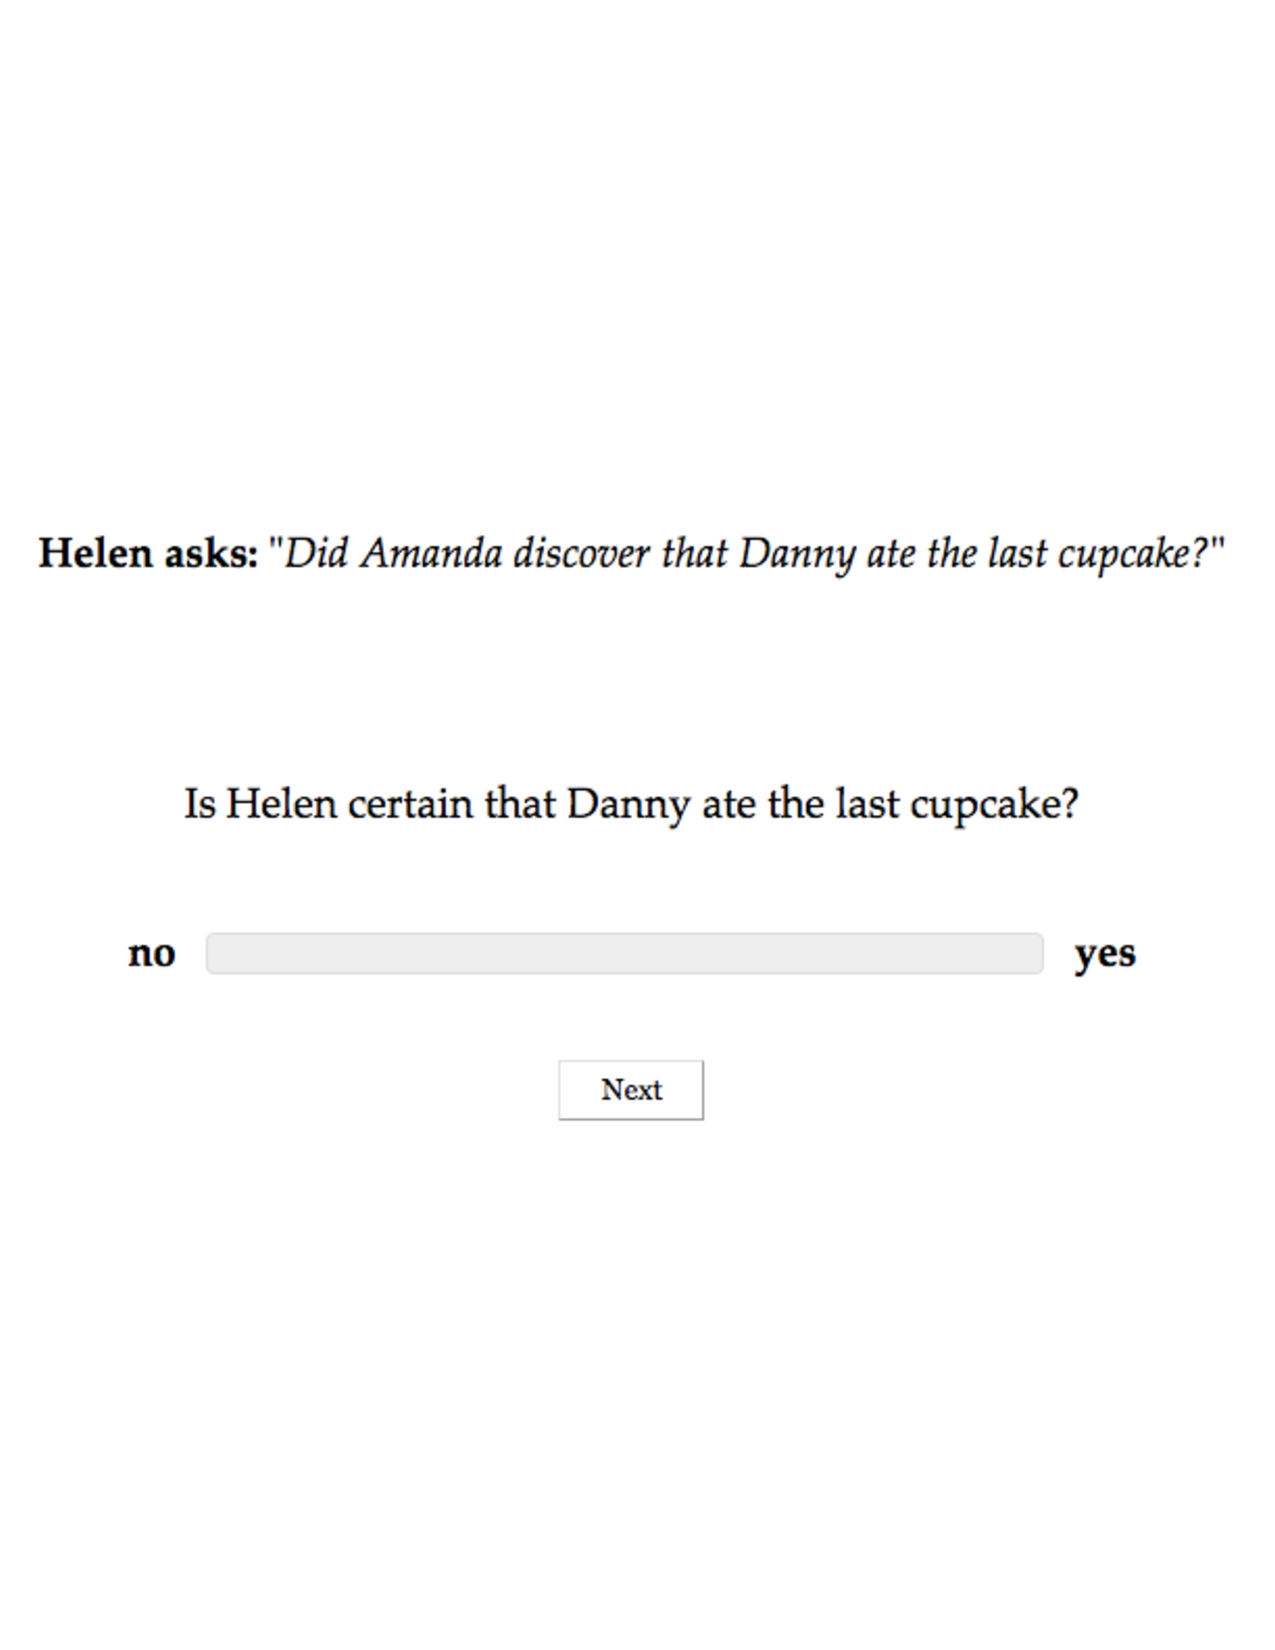
\includegraphics[width=10cm]{figures/trial-exp1}}
\end{center}
\caption{A sample trial in Experiment 1}\label{fig-trial-exp1}
\end{figure}

After completing the experiment, participants filled out a short, optional survey about their age, their gender, their native language(s) and, if English is their native language, whether they are a speaker of American English (as opposed to, e.g., Australian or Indian English). To encourage them to respond truthfully, participants were told that they would be paid no matter what answers they gave in the survey.

\paragraph{Data exclusion}
Prior to analysis, the data from 13 participants who did not self-identify as native speakers of American English were excluded. To assess whether the remaining 287 participants attended to the task, we inspected their responses to the 6 control stimuli, for which we expected low responses. We excluded the data from 16 participants whose response means on the controls were more than 2 standard deviations above the group mean. We furthermore identified 5 participants whose variance in overall response distribution was more than 2 standard deviations below the mean by-participant variance: these participants always selected roughly the same point on the response scale. We excluded the data from these 5 participants, too, leaving the data from 266 participants (ages 20-71; median: 36; 118 female, 143 male, 2 other, 3 undeclared).

\subsection{Results}

Each predicate received 266 certainty ratings and each predicate/clause combination received between 4 and 25 ratings (mean: 13.3). The plot in Figure \ref{f-projectivity} shows the mean certainty ratings for the target stimuli by predicate, collapsing over complement clauses, as well as the mean certainty rating of the main clause control stimuli (abbreviated `MC'). Participants' individual ratings are given by light gray dots. Factive predicates are given in violet, veridical non-factive predicates in blue,  projective non-factive predicates in orange and plain non-factive predicates in gray. (This color scheme is used throughout the remainder of the paper.) The mean certainty ratings are consistent with impressionistic judgments reported in the literature. First, the ratings for main clause content are lowest overall, as expected for non-projective content. Second, the ratings for factive predicates are among the highest overall, suggesting comparatively high projectivity of the content of the complement. Third, the ratings for plain non-factive predicates are among the lowest overall, suggesting comparatively low projectivity of the content of the complement. Finally, the mean certainty ratings of many of the projective non-factives are higher than those of main clauses as well as of plain non-factives, confirming the intuitions of authors like \citet{schlenker10,anand-hacquard2014} and \citet{spector-egre2015} that the content of the complement of some non-factive predicates may project.

\begin{figure}[H]
\centering

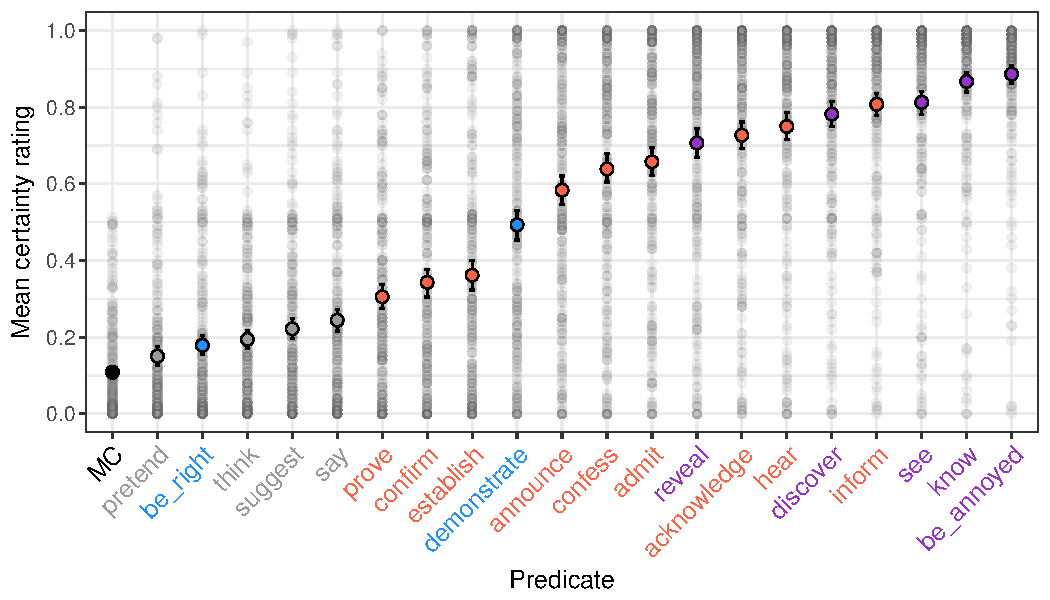
\includegraphics[width=.7\paperwidth]{../results/5-projectivity-no-fact/graphs/means-projectivity-by-predicate-variability}

\caption{Mean certainty ratings by predicate, collapsing over complement clauses, with 95\% confidence intervals. Factive predicates are given in violet, veridical non-factive ones in blue, plain non-factive ones in gray and projective non-factive ones in orange. Light gray dots indicate individual participants' responses. `MC' abbreviates main clause controls.}
\label{f-projectivity}
\end{figure}

Recall from section \ref{s1} that the distinction between factive and non-factive predicates relies on two assumptions: i) content is either projective or not, and ii) the content of the complement of factive predicates is projective whereas that of non-factive predicates, with the exception of projective non-factive predicates, is not.  Neither of these assumptions is empirically supported by the findings of Exp.~1. Regarding the first assumption, the certainty ratings plotted in Figure \ref{f-projectivity} provide further support for  \citetpos{tbd-variability} finding that projectivity is a gradient property of utterance content, not a binary categorical one.  With respect to by-predicate projection variability, we observe, for instance, that the mean certainty ratings for the contents of the complements of the 20 predicates are spread out from .17 for {\em pretend} to .86 for {\em be annoyed}, suggesting gradience in average projectivity. We also observe gradient within-predicate projection variability: for many predicates, the certainty ratings range from floor to ceiling, suggesting gradience in the extent to which participants took speakers to be committed to the content of the complement of particular clause-embedding predicates. For the factive predicate {\em reveal}, for instance, Figure \ref{f-projectivity} shows that the middle 50\% of certainty ratings fell in the range from .5 to .95. In sum, projectivity is a gradient property of utterance content, not a binary categorical one.

%14 reveal     0.688 0.0362  0.0377 0.652
%17 discover   0.763 0.0328  0.0317 0.730
%19 see        0.795 0.0314  0.0300 0.763
%20 know       0.841 0.0311  0.0263 0.810
%21 be_annoyed 0.859 0.0276  0.0263 0.831

As discussed in section \ref{s1}, the finding that projectivity is a gradient property of utterance content gives rise to the question of whether projectivity distinguishes factive predicates from non-factive ones (modulo projective non-factive ones) and how projective the content of the complement of a clause-embedding predicate needs to be in order for the predicate to be considered factive. 

{\bf UPDATED ALREADY: }
To determine which clause-embedding predicates differed from each other in the projectivity of the content of the  complement, we conducted post hoc pairwise comparisons using Tukey's method (allowing for by-participant and by-item variability), using the \verb|lsmeans| package \citep{tukey} in R \citep{r}. We included the main clause controls in the analysis to identify predicates for which the content of the complement was not projective (6916 data points total). The $p$-values for each comparison pair are shown in Table \ref{t-pairwise-proj}. 

\begin{table}[h!]
\setlength\tabcolsep{3pt}

\centering
\small

\begin{tabular}{l l l l l l l l l l l l l l l l l l l l l }
\toprule

& \rot{MC} &   \rot{\color{gray}{\em pretend}\color{black}} & \rot{\color{blue}{\em be right}\color{black}} & \rot{\color{gray}{\em think}\color{black}} &  \rot{\color{gray}{\em suggest}\color{black}} &  \rot{\color{gray}{\em say}\color{black}} & \rot{\color{orange}{\em prove}\color{black}} & \rot{\color{orange}{\em confirm}\color{black}} & \rot{\color{orange}{\em establish}\color{black}} & \rot{\color{blue}{\em demonstrate}\color{black}} & \rot{\color{orange}{\em announce}\color{black}} &\rot{\color{orange}{\em confess}\color{black}}& \rot{\color{orange}{\em admit}\color{black}} & \rot{\color{violet}{\em reveal}\color{black}}  &\rot{\color{orange}{\em acknowledge}\color{black}}  & \rot{\color{orange}{\em hear}\color{black}}  & \rot{\color{violet}{\em discover}\color{black}} & \rot{\color{orange}{\em inform}\color{black}}  & \rot{\color{violet}{\em see}\color{black}}  & \rot{\color{violet}{\em know}\color{black}}  \\

\midrule

\color{gray}{\em pretend}\color{black}	&  n.s. & - & - & - & - & - & - & - & - & - & - & - & - & - & - & - & - & - & - \\
\color{blue}{\em be right}\color{black}	& . & n.s. & - & - & - & - & - & - & - & - & - & - & - & - & - & - & - & - & - & - \\
\color{gray}{\em think}\color{black}		& ** & n.s. & n.s. & - & - & - & - & - & - & - & - & - & - & - & - & - & - & - & - & - \\
\color{gray}{\em suggest}\color{black}	& ***	& n.s. & n.s. & n.s. & - & - & - & - & - & - & - & - & - & - & - & - & - & - & - & - \\
\color{gray}{\em say}	\color{black}	& ***	& ** & n.s. & n.s. & n.s. & - & - & - & - & - & - & - & - & - & - & - & - & - & - & - \\
\color{orange}{\em prove}\color{black}		& ***	& *** &  ***  & ** & * & n.s. & - & - & - & - & - & - & - & - & - & - & - & - & - & - \\
\color{orange}{\em confirm}\color{black}	&***	& ***  &  ***  &  ***  &  ***  & ** & n.s. & - & - & - & - & - & - & - & - & - & - & - & - & - \\
\color{orange}{\em establish}\color{black}	&***	&  ***  &  ***  &  ***  &  ***  &  ***  & n.s & n.s. & - & - & - & - & - & - & - & - & - & - & - & - \\
\color{blue}{\em demonstrate}\color{black} &*** & *** & *** & *** &  *** &  *** &  ***  &  ***  &  ***  & - & - & - & - & - & - & - & - & - & - & - \\
\color{orange}{\em announce}\color{black}		& ***	& *** & *** & *** & *** & *** & *** &  ***  &  ***  & ** & - & - & - & - & - & - & - & - & - & - \\
\color{orange}{\em confess}\color{black}	& ***	& *** & *** & *** & *** & *** & *** & *** & *** &  ***  & n.s. & - & - & - & - & - & - & - & - & - \\
\color{orange}{\em admit}\color{black}		& ***	& *** & *** & *** & *** & *** & *** & *** & *** &  ***  & . & n.s. &  - & - & - & - & - & - & - & - \\
\color{violet}{\em reveal}\color{black}			& ***	& *** & *** & *** & *** & *** & *** & *** & *** &  ***  &  ***  & n.s. & n.s. & - & - & - & - & - & - & - \\
\color{orange}{\em acknowledge}\color{black}	& ***	& *** & *** & *** & *** & *** & *** & *** & *** &  ***  &  ***  & * & n.s. & n.s. & - & - & - & - & - & - \\
\color{orange}{\em hear}\color{black}		& ***	& *** & *** & *** & *** & *** & *** & *** & *** & *** &  ***  &  **  & ** & n.s. & n.s. & - & - & - & - & - \\
\color{violet}{\em discover}\color{black}	& ***		& *** & *** & *** & *** & *** & *** & *** & *** & *** &  ***  &  ***  &  ***  & . & n.s. & n.s. & - & - & - & - \\
\color{orange}{\em inform}\color{black}		&***		& *** & *** & *** & *** & *** & *** & *** & *** & *** & *** & *** &  ***  & ** & * & n.s. & n.s. & - & - & - \\
\color{violet}{\em see}\color{black}		&***		& *** & *** & *** & *** & *** & *** & *** & *** & *** & *** &  ***  &  ***  &  ***  & * & n.s. & n.s. & n.s. & - & - \\
\color{violet}{\em know}\color{black}		&***		& *** & *** & *** & *** & *** & *** & *** & *** & *** & *** & *** & *** & *** & *** & *** & * & n.s. & n.s. & -  \\
\color{violet}{\em be annoyed}\color{black}	&***		& *** & *** & *** & *** & *** & *** & *** & *** & ***  & ***  & *** & *** & *** & *** & *** & ** & * & . & ns  \\

\bottomrule
\end{tabular}
\caption{P-values associated with pairwise comparison of certainty ratings of the 20 clause-embedding predicates and the main clause controls using Tukey's method. `***' indicates significance at .0001, `**' at .01, `*' at .05, `.' marginal significance at .1, and `n.s' indicates no significant difference in means. `MC' abbreviates main clause controls. factive predicates are given in darker blue, veridical non-factive ones in lighter blue, plain non-factive ones in brown and projective non-factive ones in black.}\label{t-pairwise-proj}
\end{table} 

%# contrast                      estimate         SE     df t.ratio p.value
%# MC - pretend              -0.042020639 0.01916977  49.97  -2.192  0.8098
%# MC - be_right             -0.071607572 0.01916501  50.13  -3.736  0.0542
%# MC - think                -0.083783582 0.01916492  50.07  -4.372  0.0089
%# MC - suggest              -0.111608001 0.01912903  50.69  -5.834  0.0001
%# MC - say                  -0.133890950 0.01912899  50.72  -6.999  <.0001
%# MC - prove                -0.193307193 0.01914129  50.50 -10.099  <.0001
%# MC - confirm              -0.231812154 0.01917434  50.04 -12.090  <.0001
%# MC - establish            -0.251595754 0.01913785  50.56 -13.146  <.0001
%# MC - demonstrate          -0.381538510 0.01913109  50.66 -19.943  <.0001
%# MC - announce             -0.471695123 0.01912825  50.73 -24.660  <.0001
%# MC - confess              -0.527021744 0.01916157  50.13 -27.504  <.0001
%# MC - admit                -0.544807503 0.01912812  50.71 -28.482  <.0001
%# MC - reveal               -0.592362151 0.01912462  50.78 -30.974  <.0001
%# MC - acknowledge          -0.613560616 0.01916529  50.13 -32.014  <.0001
%# MC - hear                 -0.634910506 0.01912981  50.72 -33.190  <.0001
%# MC - discover             -0.667312302 0.01913513  50.63 -34.874  <.0001
%# MC - inform               -0.693266524 0.01915643  50.26 -36.190  <.0001
%# MC - see                  -0.697664502 0.01914503  50.43 -36.441  <.0001
%# MC - know                 -0.752791183 0.01913805  50.55 -39.335  <.0001
%# MC - be_annoyed           -0.773522289 0.01915574  50.30 -40.381  <.0001

%# pretend - be_right        -0.029586933 0.02175318 352.08  -1.360  0.9989
%# pretend - think           -0.041762942 0.02175315 351.11  -1.920  0.9404
%# pretend - suggest         -0.069587361 0.02172153 363.43  -3.204  0.1553
%# pretend - say             -0.091870311 0.02172148 363.91  -4.229  0.0051
%# pretend - prove           -0.151286554 0.02173230 359.55  -6.961  <.0001
%# pretend - confirm         -0.189791515 0.02176139 349.96  -8.721  <.0001
%# pretend - establish       -0.209575115 0.02172928 360.73  -9.645  <.0001
%# pretend - demonstrate     -0.339517871 0.02172331 362.84 -15.629  <.0001
%# pretend - announce        -0.429674484 0.02172086 363.99 -19.782  <.0001
%# pretend - confess         -0.485001104 0.02175018 352.32 -22.299  <.0001
%# pretend - admit           -0.502786864 0.02172074 363.80 -23.148  <.0001
%# pretend - reveal          -0.550341512 0.02171763 365.20 -25.341  <.0001
%# pretend - acknowledge     -0.571539977 0.02175347 351.98 -26.274  <.0001
%# pretend - hear            -0.592889867 0.02172222 363.73 -27.294  <.0001
%# pretend - discover        -0.625291662 0.02172689 361.93 -28.780  <.0001
%# pretend - inform          -0.651245884 0.02174563 354.69 -29.948  <.0001
%# pretend - see             -0.655643862 0.02173562 358.16 -30.164  <.0001
%# pretend - know            -0.710770543 0.02172942 360.62 -32.710  <.0001
%# pretend - be_annoyed      -0.731501649 0.02174507 355.26 -33.640  <.0001

%# be_right - think          -0.012176009 0.02174894 353.91  -0.560  1.0000
%# be_right - suggest        -0.040000428 0.02171732 366.37  -1.842  0.9600
%# be_right - say            -0.062283378 0.02171730 366.84  -2.868  0.3344
%# be_right - prove          -0.121699621 0.02172813 362.42  -5.601  <.0001
%# be_right - confirm        -0.160204582 0.02175720 352.72  -7.363  <.0001
%# be_right - establish      -0.179988182 0.02172509 363.62  -8.285  <.0001
%# be_right - demonstrate    -0.309930938 0.02171914 365.74 -14.270  <.0001
%# be_right - announce       -0.400087551 0.02171664 366.95 -18.423  <.0001
%# be_right - confess        -0.455414171 0.02174594 355.15 -20.942  <.0001
%# be_right - admit          -0.473199931 0.02171652 366.75 -21.790  <.0001
%# be_right - reveal         -0.520754579 0.02171338 368.20 -23.983  <.0001
%# be_right - acknowledge    -0.541953044 0.02174927 354.77 -24.918  <.0001
%# be_right - hear           -0.563302934 0.02171802 366.67 -25.937  <.0001
%# be_right - discover       -0.595704730 0.02172270 364.85 -27.423  <.0001
%# be_right - inform         -0.621658951 0.02174146 357.50 -28.593  <.0001
%# be_right - see            -0.626056929 0.02173140 361.04 -28.809  <.0001
%# be_right - know           -0.681183610 0.02172529 363.46 -31.354  <.0001
%# be_right - be_annoyed     -0.701914716 0.02174087 358.10 -32.285  <.0001

%# think - suggest           -0.027824419 0.02171720 365.42  -1.281  0.9995
%# think - say               -0.050107369 0.02171718 365.89  -2.307  0.7508
%# think - prove             -0.109523612 0.02172804 361.46  -5.041  0.0001
%# think - confirm           -0.148028572 0.02175712 351.80  -6.804  <.0001
%# think - establish         -0.167812173 0.02172500 362.66  -7.724  <.0001
%# think - demonstrate       -0.297754928 0.02171905 364.77 -13.709  <.0001
%# think - announce          -0.387911542 0.02171658 365.95 -17.862  <.0001
%# think - confess           -0.443238162 0.02174589 354.19 -20.383  <.0001
%# think - admit             -0.461023921 0.02171643 365.78 -21.229  <.0001
%# think - reveal            -0.508578569 0.02171334 367.18 -23.422  <.0001
%# think - acknowledge       -0.529777035 0.02174921 353.82 -24.358  <.0001
%# think - hear              -0.551126924 0.02171787 365.74 -25.377  <.0001
%# think - discover          -0.583528720 0.02172260 363.89 -26.863  <.0001
%# think - inform            -0.609482942 0.02174134 356.58 -28.033  <.0001
%# think - see               -0.613880920 0.02173129 360.11 -28.249  <.0001
%# think - know              -0.669007601 0.02172518 362.52 -30.794  <.0001
%# think - be_annoyed        -0.689738707 0.02174078 357.16 -31.726  <.0001

%# suggest - say             -0.022282950 0.02168553 379.04  -1.028  1.0000
%# suggest - prove           -0.081699192 0.02169639 374.37  -3.766  0.0285
%# suggest - confirm         -0.120204153 0.02172556 364.09  -5.533  <.0001
%# suggest - establish       -0.139987753 0.02169334 375.64  -6.453  <.0001
%# suggest - demonstrate     -0.269930509 0.02168737 377.89 -12.446  <.0001
%# suggest - announce        -0.360087123 0.02168490 379.13 -16.605  <.0001
%# suggest - confess         -0.415413743 0.02171425 366.68 -19.131  <.0001
%# suggest - admit           -0.433199502 0.02168475 378.95 -19.977  <.0001
%# suggest - reveal          -0.480754150 0.02168168 380.41 -22.173  <.0001
%# suggest - acknowledge     -0.501952616 0.02171755 366.31 -23.113  <.0001
%# suggest - hear            -0.523302505 0.02168625 378.86 -24.131  <.0001
%# suggest - discover        -0.555704301 0.02169097 376.91 -25.619  <.0001
%# suggest - inform          -0.581658523 0.02170974 369.17 -26.793  <.0001
%# suggest - see             -0.586056501 0.02169969 372.89 -27.008  <.0001
%# suggest - know            -0.641183182 0.02169352 375.49 -29.556  <.0001
%# suggest - be_annoyed      -0.661914288 0.02170912 369.83 -30.490  <.0001

%# say - prove               -0.059416243 0.02169635 374.86  -2.739  0.4254
%# say - confirm             -0.097921204 0.02172555 364.55  -4.507  0.0016
%# say - establish           -0.117704804 0.02169334 376.11  -5.426  <.0001
%# say - demonstrate         -0.247647560 0.02168737 378.36 -11.419  <.0001
%# say - announce            -0.337804173 0.02168484 379.66 -15.578  <.0001
%# say - confess             -0.393130793 0.02171422 367.16 -18.105  <.0001
%# say - admit               -0.410916553 0.02168471 379.46 -18.950  <.0001
%# say - reveal              -0.458471201 0.02168165 380.91 -21.146  <.0001
%# say - acknowledge         -0.479669666 0.02171752 366.79 -22.087  <.0001
%# say - hear                -0.501019556 0.02168617 379.41 -23.103  <.0001
%# say - discover            -0.533421352 0.02169092 377.43 -24.592  <.0001
%# say - inform              -0.559375573 0.02170970 369.66 -25.766  <.0001
%# say - see                 -0.563773551 0.02169966 373.39 -25.981  <.0001
%# say - know                -0.618900232 0.02169349 375.98 -28.529  <.0001
%# say - be_annoyed          -0.639631338 0.02170909 370.31 -29.464  <.0001

%# prove - confirm           -0.038504961 0.02173640 360.15  -1.771  0.9731
%# prove - establish         -0.058288561 0.02170419 371.50  -2.686  0.4651
%# prove - demonstrate       -0.188231317 0.02169820 373.73  -8.675  <.0001
%# prove - announce          -0.278387930 0.02169568 374.99 -12.831  <.0001
%# prove - confess           -0.333714550 0.02172508 362.71 -15.361  <.0001
%# prove - admit             -0.351500310 0.02169558 374.77 -16.201  <.0001
%# prove - reveal            -0.399054958 0.02169251 376.20 -18.396  <.0001
%# prove - acknowledge       -0.420253423 0.02172836 362.36 -19.341  <.0001
%# prove - hear              -0.441603313 0.02169707 374.69 -20.353  <.0001
%# prove - discover          -0.474005109 0.02170182 372.75 -21.842  <.0001
%# prove - inform            -0.499959330 0.02172053 365.19 -23.018  <.0001
%# prove - see               -0.504357308 0.02171049 368.84 -23.231  <.0001
%# prove - know              -0.559483989 0.02170436 371.35 -25.777  <.0001
%# prove - be_annoyed        -0.580215095 0.02171994 365.81 -26.713  <.0001

%# confirm - establish       -0.019783600 0.02173331 361.39  -0.910  1.0000
%# confirm - demonstrate     -0.149726356 0.02172736 363.49  -6.891  <.0001
%# confirm - announce        -0.239882969 0.02172486 364.68 -11.042  <.0001
%# confirm - confess         -0.295209590 0.02175419 352.98 -13.570  <.0001
%# confirm - admit           -0.312995349 0.02172471 364.51 -14.407  <.0001
%# confirm - reveal          -0.360549997 0.02172167 365.86 -16.599  <.0001
%# confirm - acknowledge     -0.381748462 0.02175744 352.66 -17.546  <.0001
%# confirm - hear            -0.403098352 0.02172625 364.40 -18.554  <.0001
%# confirm - discover        -0.435500148 0.02173092 362.60 -20.041  <.0001
%# confirm - inform          -0.461454369 0.02174966 355.33 -21.217  <.0001
%# confirm - see             -0.465852348 0.02173966 358.81 -21.429  <.0001
%# confirm - know            -0.520979028 0.02173343 361.29 -23.971  <.0001
%# confirm - be_annoyed      -0.541710134 0.02174904 355.95 -24.907  <.0001

%# establish - demonstrate   -0.129942756 0.02169515 375.00  -5.989  <.0001
%# establish - announce      -0.220099369 0.02169266 376.24 -10.146  <.0001
%# establish - confess       -0.275425990 0.02172202 363.93 -12.680  <.0001
%# establish - admit         -0.293211749 0.02169254 376.04 -13.517  <.0001
%# establish - reveal        -0.340766397 0.02168946 377.49 -15.711  <.0001
%# establish - acknowledge   -0.361964862 0.02172535 363.54 -16.661  <.0001
%# establish - hear          -0.383314752 0.02169403 375.97 -17.669  <.0001
%# establish - discover      -0.415716548 0.02169871 374.07 -19.159  <.0001
%# establish - inform        -0.441670769 0.02171751 366.39 -20.337  <.0001
%# establish - see           -0.446068748 0.02170745 370.08 -20.549  <.0001
%# establish - know          -0.501195428 0.02170132 372.61 -23.095  <.0001
%# establish - be_annoyed    -0.521926534 0.02171688 367.05 -24.033  <.0001

%# demonstrate - announce    -0.090156613 0.02168671 378.48  -4.157  0.0068
%# demonstrate - confess     -0.145483234 0.02171609 366.04  -6.699  <.0001
%# demonstrate - admit       -0.163268993 0.02168659 378.27  -7.529  <.0001
%# demonstrate - reveal      -0.210823641 0.02168350 379.75  -9.723  <.0001
%# demonstrate - acknowledge -0.232022106 0.02171937 365.68 -10.683  <.0001
%# demonstrate - hear        -0.253371996 0.02168808 378.19 -11.683  <.0001
%# demonstrate - discover    -0.285773792 0.02169275 376.29 -13.174  <.0001
%# demonstrate - inform      -0.311728014 0.02171154 368.55 -14.358  <.0001
%# demonstrate - see         -0.316125992 0.02170150 372.26 -14.567  <.0001
%# demonstrate - know        -0.371252672 0.02169533 374.84 -17.112  <.0001
%# demonstrate - be_annoyed  -0.391983778 0.02171092 369.20 -18.055  <.0001

%# announce - confess        -0.055326620 0.02171357 367.26  -2.548  0.5718
%# announce - admit          -0.073112380 0.02168406 379.57  -3.372  0.0981
%# announce - reveal         -0.120667028 0.02168102 381.01  -5.566  <.0001
%# announce - acknowledge    -0.141865493 0.02171682 366.93  -6.533  <.0001
%# announce - hear           -0.163215383 0.02168556 379.49  -7.526  <.0001
%# announce - discover       -0.195617179 0.02169026 377.55  -9.019  <.0001
%# announce - inform         -0.221571400 0.02170904 369.77 -10.206  <.0001
%# announce - see            -0.225969378 0.02169903 373.47 -10.414  <.0001
%# announce - know           -0.281096059 0.02169282 376.11 -12.958  <.0001
%# announce - be_annoyed     -0.301827165 0.02170843 370.42 -13.904  <.0001

%# confess - admit           -0.017785759 0.02171345 367.07  -0.819  1.0000
%# confess - reveal          -0.065340407 0.02171039 368.45  -3.010  0.2478
%# confess - acknowledge     -0.086538873 0.02174624 355.04  -3.979  0.0134
%# confess - hear            -0.107888762 0.02171498 366.96  -4.968  0.0002
%# confess - discover        -0.140290558 0.02171962 365.17  -6.459  <.0001
%# confess - inform          -0.166244780 0.02173840 357.79  -7.648  <.0001
%# confess - see             -0.170642758 0.02172837 361.32  -7.853  <.0001
%# confess - know            -0.225769439 0.02172222 363.77 -10.393  <.0001
%# confess - be_annoyed      -0.246500545 0.02173779 358.41 -11.340  <.0001

%# admit - reveal            -0.047554648 0.02168088 380.81  -2.193  0.8226
%# admit - acknowledge       -0.068753113 0.02171675 366.70  -3.166  0.1709
%# admit - hear              -0.090103003 0.02168545 379.27  -4.155  0.0068
%# admit - discover          -0.122504799 0.02169011 377.37  -5.648  <.0001
%# admit - inform            -0.148459021 0.02170898 369.52  -6.839  <.0001
%# admit - see               -0.152856999 0.02169890 373.28  -7.044  <.0001
%# admit - know              -0.207983680 0.02169272 375.88  -9.588  <.0001
%# admit - be_annoyed        -0.228714786 0.02170827 370.26 -10.536  <.0001

%# reveal - acknowledge      -0.021198465 0.02171367 368.09  -0.976  1.0000
%# reveal - hear             -0.042548355 0.02168234 380.77  -1.962  0.9275
%# reveal - discover         -0.074950151 0.02168705 378.81  -3.456  0.0768
%# reveal - inform           -0.100904373 0.02170584 370.99  -4.649  0.0009
%# reveal - see              -0.105302351 0.02169580 374.73  -4.854  0.0003
%# reveal - know             -0.160429031 0.02168964 377.33  -7.397  <.0001
%# reveal - be_annoyed       -0.181160138 0.02170524 371.63  -8.346  <.0001

%# acknowledge - hear        -0.021349890 0.02171823 366.62  -0.983  1.0000
%# acknowledge - discover    -0.053751686 0.02172293 364.79  -2.474  0.6289
%# acknowledge - inform      -0.079705907 0.02174171 357.42  -3.666  0.0400
%# acknowledge - see         -0.084103885 0.02173165 360.97  -3.870  0.0199
%# acknowledge - know        -0.139230566 0.02172545 363.46  -6.409  <.0001
%# acknowledge - be_annoyed  -0.159961672 0.02174108 358.05  -7.358  <.0001

%# hear - discover           -0.032401796 0.02169165 377.25  -1.494  0.9963
%# hear - inform             -0.058356018 0.02171044 369.47  -2.688  0.4634
%# hear - see                -0.062753996 0.02170037 373.22  -2.892  0.3186
%# hear - know               -0.117880676 0.02169422 375.79  -5.434  <.0001
%# hear - be_annoyed         -0.138611782 0.02170981 370.14  -6.385  <.0001

%# discover - inform         -0.025954222 0.02171514 367.61  -1.195  0.9998
%# discover - see            -0.030352200 0.02170507 371.33  -1.398  0.9985
%# discover - know           -0.085478881 0.02169893 373.88  -3.939  0.0154
%# discover - be_annoyed     -0.106209987 0.02171446 368.32  -4.891  0.0003

%# inform - see              -0.004397978 0.02172387 363.74  -0.202  1.0000
%# inform - know             -0.059524659 0.02171765 366.27  -2.741  0.4237
%# inform - be_annoyed       -0.080255765 0.02173323 360.85  -3.693  0.0366

%# see - know                -0.055126681 0.02170760 369.95  -2.540  0.5784
%# see - be_annoyed          -0.075857787 0.02172323 364.40  -3.492  0.0691

%# know - be_annoyed         -0.020731106 0.02171705 366.90  -0.955  1.0000

The analysis revealed that, for the most part, the content of the complement of plain non-factive and veridical non-factive predicates is less projective than that of factive and projective non-factive predicates. Critically, however, the observed by-predicate differences do not align with the assumed categorical distinction between, on the one hand, factive and projective non-factive predicates and, on the other hand, plain non-factive and veridical non-factive predicates. First, there are pairs of predicates that do not pattern as expected: the content of the complement of the veridical non-factive predicate {\em demonstrate} is more projective than that of the projective non-factive predicates {\em establish, confirm} and {\em prove}, and the content of the complement of the projective non-factive predicate {\em prove} is indistinguishable in its projectivity from that of the plain non-factive predicates {\em say} and {\em suggest}. Second, because of the observed by-predicate variability, veridical non-factive and plain non-factive predicates do not form a natural class with respect to the projectivity of the content of the complement, and neither do factive and projective non-factive predicates. That is, for the 6 veridical non-factive and plain non-factive predicates, the content of the complement of {\em demonstrate} is more projective than that of {\em be right} and of the 4 plain non-factive predicates. Likewise, for the 14 factive and projective non-factive predicates, there is widespread by-predicate variability: for instance, the content of the complement of {\em be annoyed} and {\em know} is more projective than that of {\em discover} and {\em hear}, that of {\em inform} is more projective than that of {\em acknowledge, reveal} and {\em admit}, that of {\em discover} is more projective than that of {\em reveal, admit} and {\em confess}, and that of {\em confess} is more projective than that of {\em establish}.\footnote{These findings align with those of \citealt{tbd-variability}, who also observed that the content of the complement of {\em reveal} was less projective than that of {\em discover}, which in turn was less projective than that of {\em know} and {\em be annoyed}, and that the content of {\em establish} was more projective than that of {\em confess}. There are two differences between the findings of Exp.~1 and of \citetpos{tbd-variability} Exps.~1a and 1b. First, the projectivity of the content of the complement of {\em reveal} was significantly higher than that of {\em confess} in their Exp.~1b, but it is only numerically higher in Exp.~1. Second, the certainty ratings were overall higher in \citetpos{tbd-variability} Exps.~1 than in our Exp.~1. For instance, the content of the complement of {\em be annoyed}, which was the most projective in both sets of experiments, received mean certainty ratings of .96  and .92 in their Exps.~1a and 1b, respectively, but only a .86 in our Exp.~1. Similarly, the content of the complement of {\em discover} received mean certainty ratings of .86 and .85 in their Exps.~1a and 1b, respectively, but only a .76 in our Exp.~1. Both of these differences may be due to the fact that \citet{tbd-variability} primarily explored highly projective content whereas our Exp.~1 also included a wide range of less projective content: it is possible that participants' certainty ratings were influenced by the overall projectivity of the contents explored. We leave this matter to future research.} Thus, the findings of Exp.~1 do not support the assumed binary categorical distinction between, on the one hand, factive and projective non-factive predicates, and, on the other hand, plain non-factive and veridical non-factive predicates.

Do the findings of Exp.~1 support an alternative binary categorical distinction between the 20 predicates with respect to the projectivity of the content of the complement? We argue that this is not the case. To illustrate, we note that the pairwise comparison reveals that only the content of the complement of {\em pretend} is indistinguishable in projectivity from main clause content. This finding suggests that only this content is not projective and that the content of the complement of the remaining 19 predicates, including that of the other 3 plain non-factive and the 2 veridical non-factive predicates, can be considered at least weakly projective.\footnote{\citet{spector-egre2015} suggested that it is not clear whether the content of the complement of {\em say} is projective (p.1739) but that it is definitely less projective than that of {\em tell}. The findings of Exp.~1 suggest that it is very weakly projective.} Now consider an alternative binary categorical division among the 20 clause-embedding predicates: the first set consists of {\em pretend, be right, think, suggest} and {\em say}, i.e., the 5 predicates for which the content of the complement is least projective, and the second set of the remaining 15 predicates. Neither of the two sets of predicates forms a natural class: the first set includes predicates for which the content of the complement is not projective as well as predicates for which it is weakly projective, and the second set includes predicates that exhibit significant differences in the projectivity of the content of the complement. Furthermore, the projectivity of the content of the complement of {\em say} and {\em suggest} (first set) is indistinguishable from that of {\em prove} (second set), which illustrates the arbitrariness of the dividing line. More generally, we argue that any binary categorical distinction between the 20 predicates is bound to be arbitrary because of the rampant by-predicate variability and the observation that the content of the complement of most of these 20 predicates is at least weakly projective.

In sum, Exp.~1 confirmed \citetpos{tbd-variability} finding that projectivity is a gradient property of utterance content and showed that projectivity does not categorically distinguish the content of the complement of factive (and projective non-factive) predicates from that of `(plain and veridical) non-factive' predicates. The experiments described in the next section were designed to explore whether the content of the complement of the same 20 clause-embedding predicates is entailed, to identify whether entailment and projectivity jointly distinguish factive and non-factive predicates, as per the definition in (\ref{def}).


\subsection{Discussion}

- projectivity alone does not distinguish factive from non-factive predicates: no non-arbitrary cut-off point
 
\section{Experiment 2: Entailment}\label{s3}

The two experiments described in this section were designed explore whether the content of the complement is entailed by the content of unembedded matrix sentences with the 20 clause-embedding predicates. We assume a standard definition of entailment, according to which entailment is a binary, categorical relation between two contents: given sentences $\phi$ and $\psi$, the content of $\phi$ entails the content of $\psi$ if and only if every world in which the content of $\phi$ is true is also a world in which the content of $\psi$ is true. Thus, if there is even one world in which $\phi$ is true but $\phi$ is false, then the content of $\phi$ does not entail the content of $\psi$. 

Given this standard definition of the entailment relation, it is straightforward to establish that the contents of two natural language sentences $\phi$ and $\psi$ do not stand in an entailment relation, namely by identifying a world in which the content of $\phi$ is true and the content of $\psi$ is false. In this paper, however, we are also interested in establishing that the contents of two sentences $\phi$ and $\psi$  stand in an entailment relation. Establishing this is straightforward if the content of some expression in $\phi$ denotes a subset of the content of some expression in $\psi$: for instance, in (\ref{ent1}a),  the content of $\phi$ entails the content of $\psi$ because the denotation of {\em black cat} in $\phi$ is a subset of the denotation of {\em cat} in $\psi$. No such structural relation exists, however, between the content of a sentence with a clause-embedding predicate and the content of the complement, as in (\ref{ent1}b). Furthermore, it is impossible to empirically verify that the content of $\phi$ entails the content of $\psi$ in (\ref{ent1}b) because it is impossible to verify that $\psi$ is true in all worlds in which $\phi$ is true. 

\begin{exe}
\ex\label{ent1}
\begin{xlist}
\ex $\phi$: Sam owns a black cat. \hspace*{1.5cm} $\psi$: Sam owns a cat.

\ex $\phi$: Sam knows that it's raining. \hspace*{.6cm} $\psi$: It's raining.

\end{xlist}
\end{exe}

Thus, to establish whether the content of an unembedded matrix sentence with a clause-embedding predicate entails the content of the clausal complement, we resort to diagnostics that are taken to provide evidence for an entailment relation. Two standard diagnostics are given in (\ref{diag}); these were already illustrated with the emotive predicate {\em regret} in section \ref{s1}. According to the `inference diagnostic' in (\ref{diag}a), the content of an unembedded matrix sentence with a clause-embedding predicate entails the content of the complement if and only if the content of the complement definitely follows from a true statement of the unembedded matrix sentence. {\bf  ONLY A NECESSARY CONDITION, NOT SUFFICIENT} According to the `contradictoriness diagnostic' in (\ref{diag}b), such an entailment relationship holds if and only an utterance of the unembedded matrix sentence that is followed by a denial of the content of the complement is contradictory. 

\begin{exe}
\ex\label{diag} Two diagnostics for entailment \hfill (see, e.g., \citealt[\S3.1]{ccmg90})
\begin{xlist}
\ex  Inference diagnostic \\ $\phi$ entails $\psi$ if and only if, if $\phi$ is true, then the truth of $\psi$ definitely follows. 

\ex  Contradictoriness diagnostic \\ $\phi$ entails $\psi$ if and only if sentences of the form {\em $\phi$ and not $\psi$} are contradictory. 

\end{xlist}
\end{exe}
These two diagnostics for entailment are applied to the content of the complement of the 20 clause-embedding predicates in Exps.~2a and 2b, respectively. Both experiments include control stimuli for which the relevant inference definitely follows (Exp.~2a) and that are definitely contradictory (Exp.~2b). We assume that the content of the clausal complement of sentences with a clause-embedding predicate is not an entailment if responses to the content of the clausal complement are significantly different from responses to the control stimuli. According to the diagnostics, identifying contents of clausal complements that are entailments, however, requires arguing from a null result: the content of the complement of sentences with a clause-embedding predicate is an entailment if responses to the content of the complement are not significantly different from responses to the control stimuli. We present the findings of the two experiments in sections \ref{s31} and \ref{s32}, and then discuss the findings jointly in section \ref{s33}.

\subsection{Experiment 2a: Inference diagnostic for entailment}\label{s31}

This experiment explored whether the content of the clausal complement of the 20 clause-embedding predicates is an entailment based on the inference diagnostic for entailment in (\ref{diag}a). In contrast to the entailment relationship, which is binary and categorical, the inference relationship between the contents of two sentences $\phi$ and $\psi$ is gradient: given a true statement $\phi$, the truth of $\psi$ follows to varying degrees. To illustrate, assume that Chris wears his pajamas whenever he is at home and that he doesn't wear pajamas outside of his home. Now consider the contents of the sentences $\phi_1$ to $\phi_5$ in (\ref{chris}). Given the aforementioned assumption, the (truth of the) content of the statement $\psi$ {\em Chris is wearing his pajamas} definitely follows from a true statement of $\phi_1$, it follows to increasingly lower degrees from true statements of $\phi_2$ to $\phi_4$ and it definitely does not follow from a true statement of $\phi_5$. 

\begin{exe}
\ex\label{chris}
\begin{xlist}
\exi{$\phi_1$} Chris is at home.
\exi{$\phi_2$} Chris is likely at home.
\exi{$\phi_3$} Chris is possibly at home.
\exi{$\phi_4$} There is a slight possibility that Chris is at home.
\exi{$\phi_5$} Chris is not at home.
\end{xlist}
\end{exe}

In applying the inference diagnostic for entailment in Exp.~2a, we assume that if the content of $\phi$ entails the content of $\psi$, then the (truth of the) content of $\psi$ definitely follows from true statements of $\phi$, i.e., the strength of the inference is at ceiling. If the content of $\phi$ does not entail the content of $\psi$, then the strength of the inference is somewhere below ceiling. Exp.~2a investigated the strength of the inference from true statements of unembedded matrix sentences with the 20 clause-embedding predicates to the contents of the complements by collecting gradient inference ratings.

\subsubsection{Methods}

\paragraph{Participants} 300 participants with U.S.\ IP addresses and at least 99\% of previous HITs approved were recruited on Amazon's Mechanical Turk platform (ages: 19-69, median: 36; 152 female, 148 male). They were paid 75 cents for participating in the experiment.

\paragraph{Materials} The target stimuli were 400 unembedded matrix sentences that were constructed by combining the 400 predicate/clause combinations of Exp.~1 with a random proper name subject whose gender differed from the gender of the proper name subject of the embedded clause. As illustrated in the sample stimuli in (\ref{stims2}), these matrix sentences were presented to participants as true statements. For each of the 400 target stimuli, the inference that was tested was the inference to the content of the clausal complement: for instance, participants were asked about (\ref{stims2}a) whether it follows that Danny ate the last cupcake and about (\ref{stims2}b) whether it follows that Emma studied on Saturday morning.

\begin{exe}
\ex\label{stims2}
\begin{xlist}
\ex {\bf What is true:} Melissa knows that Danny ate the last cupcake.
%\\ Does it follow that Danny ate the last cupcake?
\ex {\bf What is true:} Jerry pretended that Emma studied on Saturday morning.
%\\ Does it follow that Emma studied on Saturday morning?
\end{xlist}
\end{exe}

The experiment also included eight control stimuli that were used to assess whether participants were attending to the task, whether they interpreted the task correctly, as well as to identify inference ratings that were at ceiling and at floor. For the four entailing control stimuli in (\ref{control-good2}), the tested inferences are lexical entailment of the true statements: for instance, that Frederick solved the problem is a lexical entailment of the true statement in (\ref{control-good2}a) that Frederick managed to solve the problem and that the window broke is a lexical entailment of the true statement in (\ref{control-good2}b) that Tara broke the window with a bat. We expected the inference ratings for these lexical entailments to be at ceiling, i.e., to be entailments. In contrast, the inferences tested with the four non-entailing control stimuli in (\ref{control-bad2}) definitely do not follow from these true statements: in (\ref{control-bad2}a), that Dana wears a wig does not follow from Dana watching a movie last night, and that Madison closed the window is the negation of what actually follows from the true statement in (\ref{control-bad2}c). We expected the inference ratings for these four control stimuli to be at floor.

\begin{exe}
\ex\label{control-good2} Entailing control stimuli
\begin{xlist}
\ex {\bf What is true:} Zack bought himself a car this morning. (Tested inference: Zack owns a car.)
\ex {\bf What is true:} Tara broke the window with a bat. (Tested inference: The window broke.)
\ex {\bf What is true:} Frederick managed to solve the problem. (Tested inference: Frederick solved the problem.)
\ex {\bf What is true:} Vanessa happened to look into the mirror. (Tested inference: Vanessa looked into the mirror.)
\end{xlist}
\ex\label{control-bad2} Non-entailing control stimuli
\begin{xlist}
\ex {\bf What is true:} Dana watched a movie last night. (Tested inference: Dana wears a wig.)
\ex {\bf What is true:} Hendrick is renting an apartment. (Tested inference: The apartment has a balcony.)
\ex {\bf What is true:} Madison was unsuccessful in closing the window. (Tested inference:  Madison closed the window.)
\ex {\bf What is true:} Sebastian failed the exam. (Tested inference: Sebastian did really well on the exam.)
\end{xlist}
\end{exe}

Each participant saw a random set of 28 stimuli: each set contained one target stimulus for each of the 20 predicates (each with a unique complement clause) and the same 8 control stimuli. Trial order was randomized.

\paragraph{Procedure} Participants were told that they would read true statements and that they would be asked to assess whether a second statement follows from the first, true statement. On each trial, participants read the true statement and were asked to respond to the question {\em Does it follow that\ldots} where the continuation was realized by the complement of the clause-embedding predicate. Participants gave their responses on a sliding scale from `definitely doesn't follow' (coded as 0) to `definitely follows' (coded as 1), as shown in Figure \ref{f-trial-exp3}.

\begin{figure}[H]
\begin{center}
\fbox{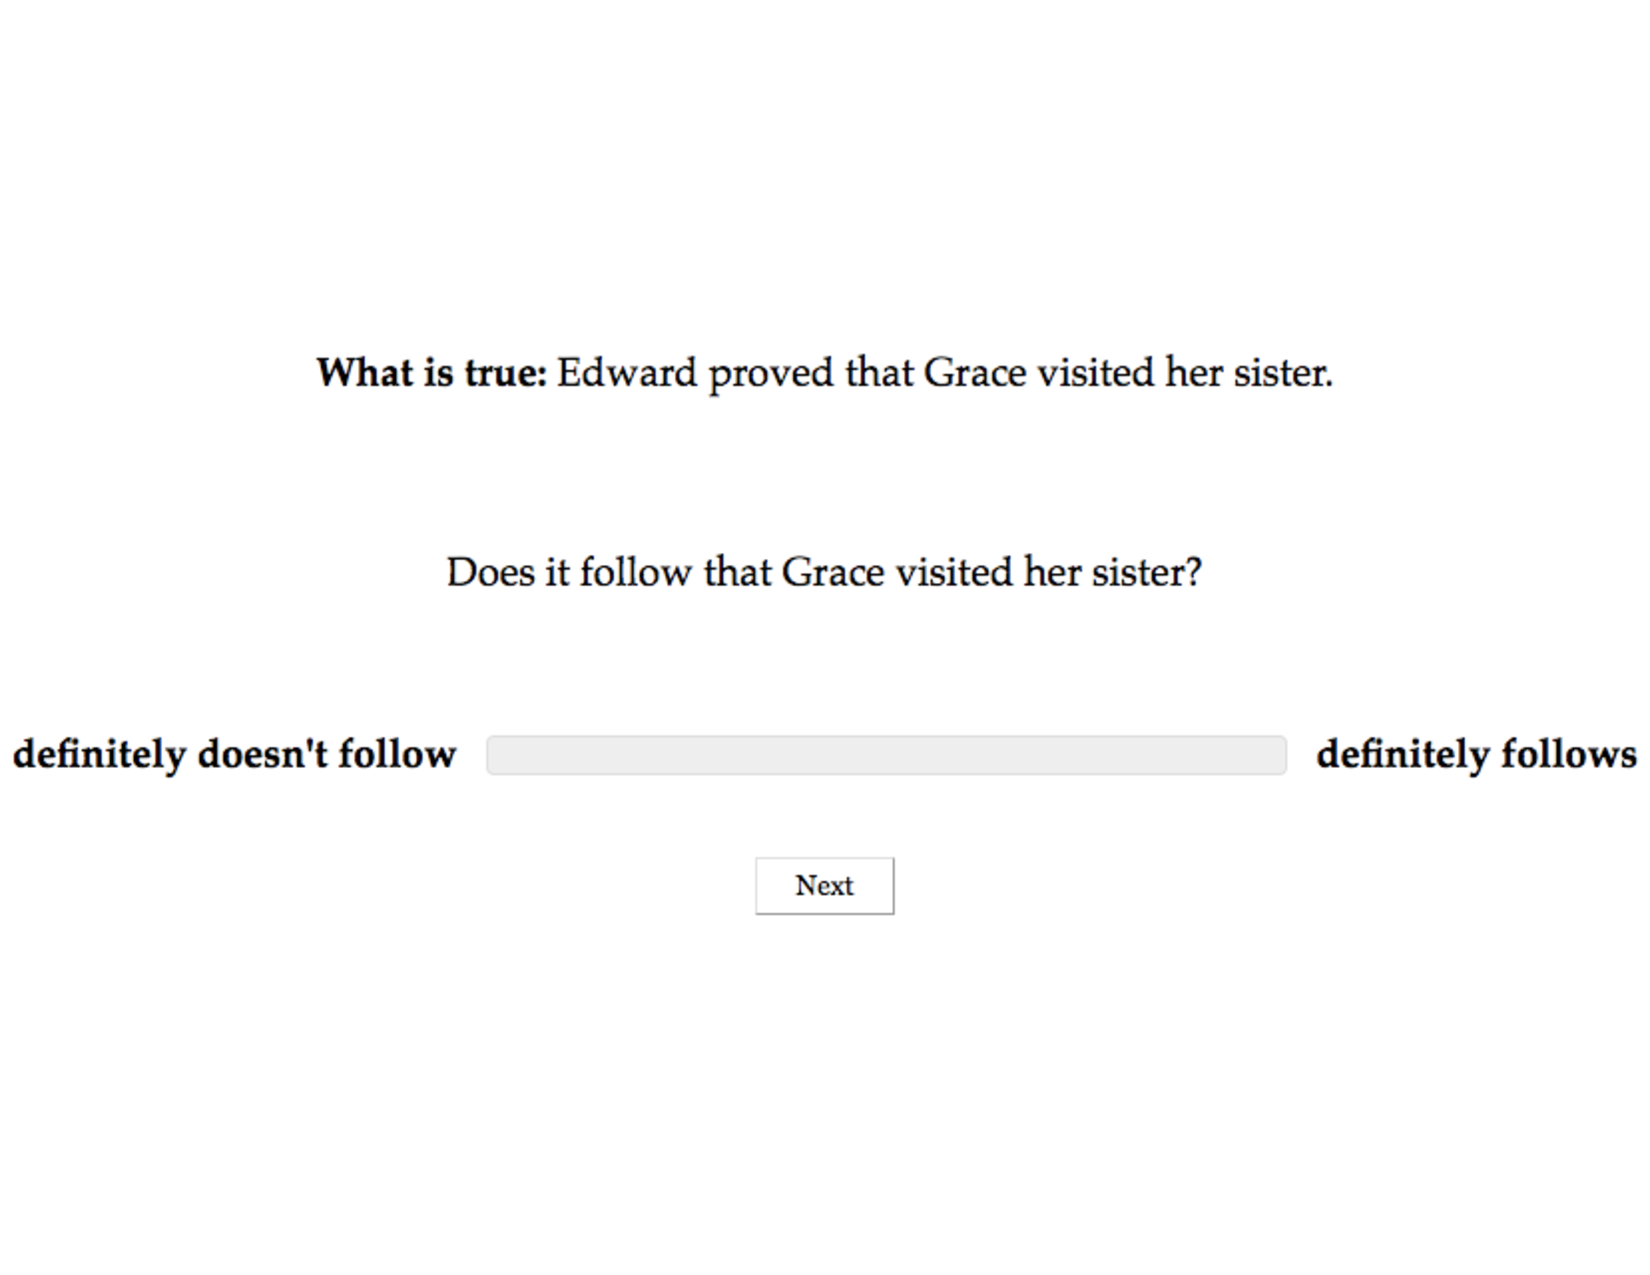
\includegraphics[width=13cm]{figures/inference-trial}}
\end{center}
\caption{A sample trial in Experiment 2a}\label{f-trial-exp3}
\end{figure}

To familiarize participants with the task, they first responded to the two familiarization stimuli in (\ref{train2}), where the inference tested was the inference to the content of the clausal complement. Participants who rated (\ref{train2}a) in the lower half of the sliding scale or (\ref{train2}b) in the upper half of the sliding scale were given an explanation for why their answer was wrong. Participants could only advance to the 28 stimuli if they gave a plausible rating to the two familiarization stimuli, i.e., a rating in the upper half of the sliding scale for (\ref{train2}a) and in the lower half for (\ref{train2}b).

\begin{exe}
\ex\label{train2}
\begin{xlist}
\ex {\bf What is true:} Drew is correct that Patty lives in Canada. 

\ex {\bf What is true}: Drew believes that Patty lives in Canada.
\end{xlist}
\end{exe}

After responding to the 28 stimuli, participants filled out a short, optional survey about their age, their gender, their native language(s) and, if English is their native language, whether they are a speaker of American English (as opposed to, e.g., Australian or Indian English). To encourage them to respond truthfully, participants were told that they would be paid no matter what answers they gave in the survey.

\paragraph{Data exclusion}

Prior to analysis, the data from 14 participants who did not self-identify as native speakers of American English were excluded. For the remaining 286 participants, we inspected their responses to the 8 control stimuli. The group means for the four control stimuli in (\ref{control-good2}), for which the strength of the inference was expected to be at ceiling, was .94. The group mean for the four control stimuli in (\ref{control-bad2}), for which the strength of the inference was expected to be at floor, was .05. These group means suggest that, overall, participants attended to and understood the task. The response means of 27 participants were more than 2 standard deviations below the group mean for the control stimuli in (\ref{control-good2}) or above the group mean for the control stimuli in (\ref{control-bad2}). Closer inspection revealed that these participants' responses to the control stimuli were systematically higher or lower, respectively, suggesting that these participants did not attend to the task or interpreted the task differently. The data from these 27 participants were also excluded. In this experiment, we did not identify any participants who always selected roughly the same point on the response scale. The results presented below are based on data from 259 participants (ages 19-69; median: 36; 132 female, 128 male); the group means were .96 for the control stimuli in (\ref{control-good2}) and .03 for the control stimuli in (\ref{control-bad2}).

\subsubsection{Results}

Each of the 20 clause-embedding predicates received 259 ratings and each of the 400 predicate/clause combinations received between 3 and 23 ratings (mean: 13). The plot in Figure \ref{f-veridicality-predicate2} shows the mean inference ratings for the target stimuli by predicate, collapsing over complement clauses, as well as the mean inference ratings of the non-entailing controls (abbreviated `non-ent. C') and the entailing controls (abbreviated `entailing C'). Participants' individual ratings are given by light gray dots. Factive predicates are given in violet, veridical non-factive predicates in blue,  projective non-factive predicates in orange and plain non-factive predicates in gray. The plain non-factive predicates {\em pretend, think, suggest} and {\em say} received among the lowest ratings overall, as expected from the assumption that the content of the complement of these predicates is not entailed.  The mean inference ratings of several predicates were at or close to ceiling (recall the group mean of .96 for the entailing control stimuli in (\ref{control-good2})), including the factive predicates {\em see} (.95), {\em discover} (.94),  {\em know} (.93), {\em be annoyed} (.92) and {\em reveal} (.9), as well as the veridical non-factive predicate {\em be right} (.96), but also the projective non-factive predicates {\em prove} (.96),  {\em establish} (.90), {\em admit} (.91), and {\em acknowledge} (.91). This finding suggests that participants took the truth of the content of the clausal complement of these predicates to (mostly) follow from the true statements of unembedded matrix sentences with these predicates. {\bf NECESSARY, NOT SUFFICIENT} The same holds for the purported veridical non-factive predicate {\em demonstrate}, whose mean inference rating was not at ceiling (.85). 

% 1 acknowledge 0.905  0.0182  0.0161 
% 2 admit       0.907  0.0207  0.0177 
% 3 announce    0.809  0.0296  0.0296 
% 4 be_annoyed  0.924  0.0160  0.0151 
% 5 be_right    0.955  0.0116  0.0106 
% 6 confess     0.890  0.0209  0.0186 
% 7 confirm     0.943  0.0115  0.0109 
% 8 demonstrate 0.854  0.0266  0.0246 
% 9 discover    0.944  0.00936 0.00932
%10 entailing C 0.961  0.00443 0.00410
%11 establish   0.903  0.0205  0.0191 
%12 hear        0.498  0.0402  0.0412 
%13 inform      0.833  0.0285  0.0266 
%14 know        0.931  0.0155  0.0134 
%15 non-ent. C  0.0297 0.00404 0.00429
%16 pretend     0.116  0.0268  0.0290 
%17 prove       0.956  0.0109  0.0102 
%18 reveal      0.903  0.0195  0.0172 
%19 say         0.683  0.0366  0.0390 
%20 see         0.948  0.0114  0.0102 
%21 suggest     0.343  0.0354  0.0363 
%22 think       0.316  0.0342  0.0330

\begin{figure}[h!]
\centering

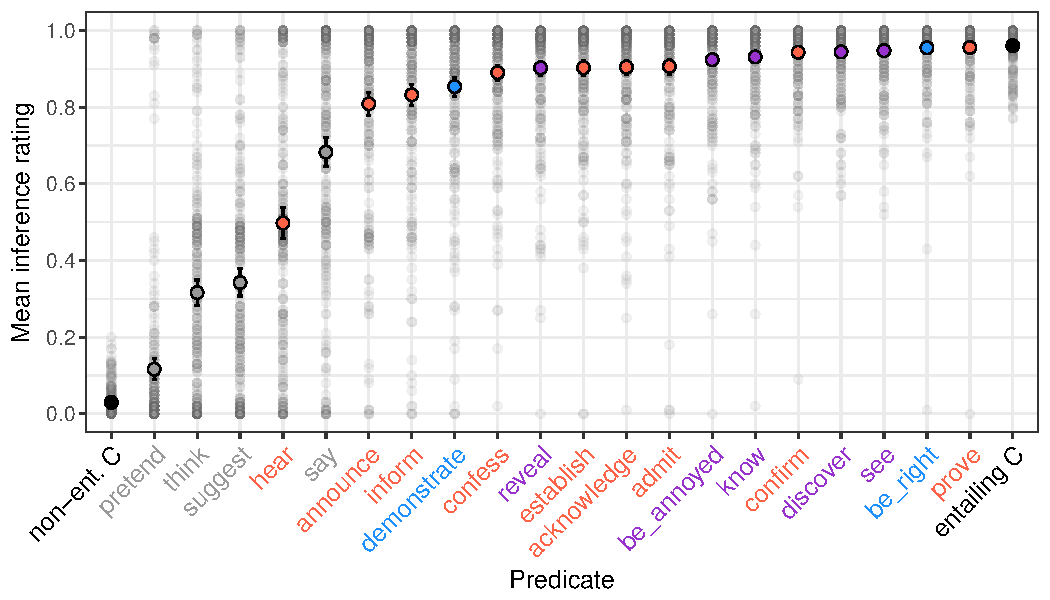
\includegraphics[width=.7\paperwidth]{../results/4-veridicality3/graphs/means-inference-by-predicate-variability}

\caption{Mean inference rating by predicate, collapsing over complements, including the non-entailing controls (`non-ent.\ C') and the entailing controls (`entailing C'). Error bars indicate 95\% confidence intervals. Light gray dots indicate individual participants' ratings. Factive predicates are given in violet, veridical non-factive ones in blue, projective non-factive ones in orange and plain non-factive ones in gray.}
\label{f-veridicality-predicate2}
\end{figure}

To determine which clause-embedding predicates are such that the content of the complement is entailed, i.e., for which clause-embedding predicates the strength of the inference to the content of the complement is at ceiling, we fit a Bayesian model predicting rating from predicate. Random effects for item and participant. slope for verb for the by-participant random effect

Results: which ones are indistinguishable from entailing controls?

Not significantly different from entailing controls: {\em be right}, {\em confirm}, {\em discover}, {\em prove}, {\em see}


%\begin{table}[h!]
%\setlength\tabcolsep{3pt}
%
%\centering
%\small
%
%\begin{tabular}{l l l l l l l l l l l l l l l l l l l l l }
%\toprule
%
% &  \rot{\color{brown}{\em pretend}\color{black}} & \rot{\color{brown}{\em think}\color{black}} & \rot{\color{brown}{\em suggest}\color{black}} &  \rot{\color{black}{\em hear}\color{black}} &  \rot{\color{brown}{\em say}\color{black}} & \rot{{\em announce}} & \rot{{\em inform}} & \rot{\color{airforceblue}{\em demonstrate}\color{black}} & \rot{\color{black}{\em confess}\color{black}} & \rot{\color{blue}{\em reveal}\color{black}} & \rot{{\em acknowledge}} & \rot{{\em admit}} & \rot{\color{black}{\em establish}\color{black}}  & \rot{\color{blue}{\em be annoyed}\color{black}}  & \rot{\color{blue}{\em know}\color{black}}  & \rot{\color{black}{\em confirm}\color{black}} & \rot{\color{blue}{\em discover}\color{black}}  & \rot{\color{blue}{\em see}\color{black}}  & \rot{\color{airforceblue}{\em be right}\color{black}} & \rot{\color{black}{\em prove} \color{black}}  \\
%\midrule
%
%\color{brown}{\em think}\color{black}		& *** & - & - & - & - & - & - & - & - & - & - & - & - & - & - & - & - & - & - & -\\
%\color{brown}{\em suggest}\color{black}			& *** & n.s. & - & - & - & - & - & - & - & - & - & - & - & - & - & - & - & - & - & - \\
%\color{black}{\em hear}	\color{black}		& *** & *** & *** & - & - & - & - & - & - & - & - & - & - & - & - & - & - & - & - & -\\
%\color{brown}{\em say}\color{black}		& *** & *** & *** & *** & - & - & - & - & - & - & - & - & - & - & - & - & - & - & - & -\\
%\color{black}{\em announce}\color{black}		& *** & *** & *** & *** & *** & - & - & - & - & - & - & - & - & - & - & - & - & - & - & -\\
%\color{black}{\em inform}\color{black}		& *** & *** & *** & *** & *** & n.s. & - & - & - & - & - & - & - & - & - & - & - & - & - & -\\
%\color{airforceblue}{\em demonstrate}\color{black}		& *** & *** & *** & *** & *** & n.s. & n.s. & - & - & - & - & - & - & - & - & - & - & - & - & -\\
%\color{black}{\em confess}\color{black}		& *** & *** & *** & *** & *** & *** & * & n.s. & - & - & - & - & - & - & - & - & - & - & - & -\\
%\color{blue}{\em reveal}\color{black}		& *** & *** & *** & *** & *** & *** & ** & * & n.s. & - & - & - & - & - & - & - & - & - & - & -\\
%\color{black}{\em acknowledge}\color{black}	& *** & *** & *** & *** & *** & *** & ** & * & n.s. & n.s. & - & - & - & - & - & - & - & - & - & -\\
%\color{black}{\em admit}\color{black}			& *** & *** & *** & *** & *** & *** & ** & * & n.s. & n.s. & n.s. & - & - & - & - & - & - & - & - & -\\
%\color{black}{\em establish}\color{black}		& *** & *** & *** & *** & *** & *** & ** & * & n.s. & n.s. & n.s. &  ns & - & - & - & - & - & - & - & -\\
%\color{blue}{\em be annoyed}\color{black}	& *** & *** & *** & *** & *** & *** & *** & ** & n.s. & n.s. & n.s. & n.s. & n.s. & - & - & - & - & - & - & -\\
%\color{blue}{\em know}\color{black}		& *** & *** & *** & *** & *** & *** & *** & *** & n.s. & n.s. & n.s. & n.s. & n.s. & n.s. & - & - & - & - & - & -\\
%\color{black}{\em confirm}\color{black}		& *** & *** & *** & *** & *** & *** & *** & *** & * & n.s. & n.s. & n.s. & n.s. & n.s. & n.s. & - & - & - & - & -\\
%\color{blue}{\em discover}\color{black}			& *** & *** & *** & *** & *** & *** & *** & *** & * & n.s. & n.s. & n.s. & n.s. & n.s. & n.s. & n.s. & - & - & - & -\\
%\color{blue}{\em see}\color{black}			& *** & *** & *** & *** & *** & *** & *** & *** & ** & n.s. & n.s. & n.s. & n.s. & n.s. & n.s. & n.s. & n.s. & - & - & - \\
%\color{airforceblue}{\em be right}\color{black}			& *** & *** & *** & *** & *** & *** & *** & *** & ** & * & . & . & . & n.s. & n.s. & n.s. & n.s. & n.s. & - & - \\
%\color{black}{\em prove}\color{black}		& *** & *** & *** & *** & *** & *** & *** & *** & **  & *  & * & * & * & n.s. & n.s. & n.s. & n.s. & n.s. & n.s. & - \\
%\color{black}controls (\ref{control-good2})\color{black}		& *** & *** & *** & *** & *** & *** & *** & *** & ***  & ** & ** & ** & ** & . & n.s. & n.s. & n.s. & n.s. & n.s.  & n.s. \\
%
%\bottomrule
%\end{tabular}
%\caption{P-values associated with pairwise comparison of inference ratings of the 20 clause-embedding predicates and the entailing controls in (\ref{control-good2}) using Tukey's method. `***' indicates significance at .0001, `**' at .01, `*' at .05, `.' marginal significance at .1, and `n.s.' indicates no significant difference in means. factive predicates are given in darker blue, veridical non-factive ones in lighter blue, non-factive ones in brown and `apparently factive' ones in black.}\label{t-pairwise2}
%\end{table}


\subsection{Experiment 2b: Contradictoriness diagnostic for entailment}\label{s32}

This experiment explored whether the content of the complement of the 20 clause-embedding predicates is an entailment based on the contradictoriness diagnostic for entailment in (\ref{diag}b). Participants rated the contradictoriness of utterances of English sentences of the form {\em $\phi$ but not $\psi$}, where $\phi$ is an unembedded matrix sentence with a clause-embedding predicate and $\psi$ is its clausal complement. We collected gradient rather than binary contradictoriness ratings because we anticipated that participants' assessment of the contradictoriness of a speaker's utterance may depend on contextual factors: for instance, we assume that the extent to which  an utterance of the sentence in (\ref{announce3}) with the projective non-factive predicate {\em announce} is contradictory may depend on how trustworthy Mary is. 

\begin{exe}
\ex\label{announce3} Mary announced that she is pregnant, but she's not.
\end{exe}
We assume that when the content of $\phi$ entails the content of $\psi$, the contradictoriness of an utterance of the form {\em $\phi$ but not $\psi$} is not mitigated by contextual factors, and participants' contradictoriness ratings will be at ceiling. If, however, the contradictoriness of an utterance of the form {\em $\phi$ but not $\psi$} is mitigated by contextual factors, then the content of $\phi$ does not entail the content of $\psi$, and participants' contradictoriness ratings will be somewhere below ceiling.

\subsubsection{Methods}

\paragraph{Participants} 300 participants with U.S.\ IP addresses and at least 99\% of previous HITs approved were recruited on Amazon's Mechanical Turk platform (ages: 18-72, median: 35; 137 female, 162 male, 1 other). They were paid 75 cents for participating in the experiment.

\paragraph{Materials} In the target stimuli, the 400 predicate/clause combinations were combined with a random proper name subject and a {\em but-}clause that denied the truth of the content of the clausal complement. As shown by the sample stimuli in ({\ref{stims}), the target stimuli were presented to participants as utterances by named speakers. The proper names that realized the speakers, the subjects of the 20 predicates and the subjects of the complement clauses were all unique. The gender of the proper name subject of the predicate was distinct from the gender of the proper name in the complement clause, to ensure that the pronoun in the elliptical {\em but-}clause unambiguously referred to the individual referred to in the complement clause of the predicate.

\begin{exe}
\ex\label{stims}
\begin{xlist}
\ex {\bf Christopher:} {\em ``Melissa knows that Danny ate the last cupcake, but he didn't.''}
\ex {\bf Susan:} {\em ``Jerry pretended that Emma studied on Saturday morning, but she didn't.}
\end{xlist}
\end{exe}

The experiment also included eight control stimuli that were used to assess whether participants were attending to the task, whether they interpreted the task correctly, as well as to identify inference ratings that were at ceiling and at floor. (These stimuli were also presented to the participants as utterances by named speakers.) For the four non-contradictory control stimuli in (\ref{control-good}), we expected contradictoriness ratings at floor because the content of the second clause does not contradict the content of the first clause: for instance, in (\ref{control-good}d), the content that Vanessa is good at math does not entail the negation of the content that the speaker is not good at math. In contrast, we expected contradictoriness ratings at ceiling for the four contradictory control stimuli in (\ref{control-bad}) because the first clause of each of these stimuli entails the negation of the second clause: in (\ref{control-bad}c), for instance, the content of {\em Madison laughed loudly} entails that Madison laughed, i.e., the negation of {\em she didn't laugh}.

\begin{exe}
\ex\label{control-good} Non-contradictory control stimuli
\begin{xlist}
\ex Zack believes that I'm married, but I'm actually single.
\ex Tara wants me to cook for her and I'm a terrific cook.
\ex Frederick is both smarter and taller than I am.
\ex Vanessa is really good at math, but I'm not.
\end{xlist}
\ex\label{control-bad} Contradictory control stimuli
\begin{xlist}
\ex Dana has never smoked in her life and she stopped smoking recently.
\ex Hendrick's car is completely red and his car is not red.
\ex Madison laughed loudly and she didn't laugh.
\ex Sebastian lives in the USA and has never been to the USA.
\end{xlist}
\end{exe}

Each participant saw a random set of 28 stimuli: each set contained one target stimulus for each of the 20 predicates (each with a unique complement clause) and the same 8 control stimuli. Trial order was randomized.


\paragraph{Procedure.} Participants were told that they would read utterances made by a speaker and were asked to assess whether the speaker's utterance is contradictory. On each trial, participants read the speaker's utterance and then gave their response on a slider marked `definitely no' at one end (coded as 0) and `definitely yes' at the other (coded as 1), as shown in Figure \ref{f-trial-exp2}.

\begin{figure}[h!]
\begin{center}
\fbox{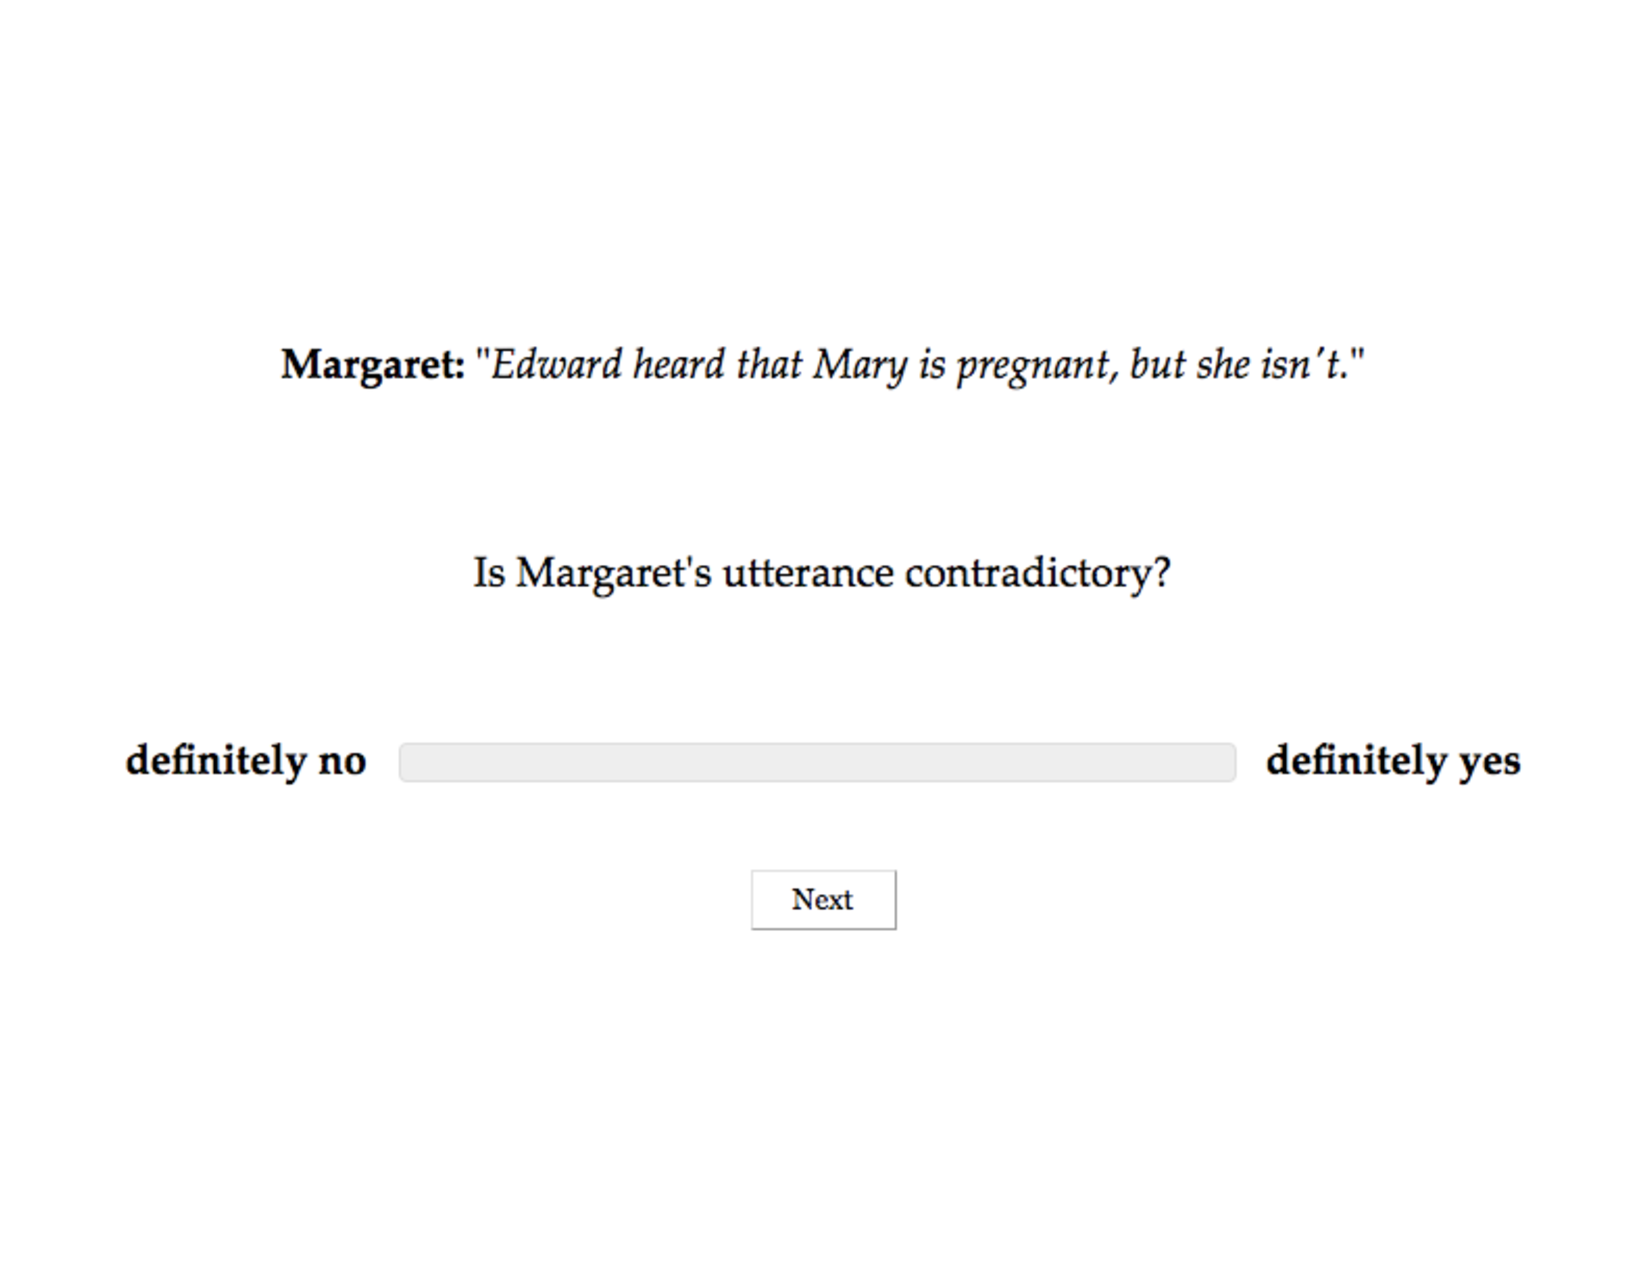
\includegraphics[width=13cm]{figures/contradictory-trial}}
\end{center}
\caption{A sample trial in Experiment 2b}\label{f-trial-exp2}
\end{figure}

To familiarize participants with the task, they first responded to the two familiarization stimuli in (\ref{train}): participants who rated (\ref{train}a) in the lower half of the scale or (\ref{train}b) in the upper half of the scale were given an explanation for why their answer was wrong. Participants could only advance to the 28 stimuli if they gave a plausible rating to the two training stimuli, i.e., a rating in the upper half of the scale for (\ref{train}b) and a rating in the lower half of the scale for (\ref{train}b).

\begin{exe}
\ex\label{train}
\begin{xlist}
\ex Drew is aware that Patty lives in Canada, but she doesn't.

\ex Drew thinks that Patty lives in Canada, but she doesn't.
\end{xlist}
\end{exe}

After responding to the 28 stimuli, participants filled out a short, optional survey about their age, their gender, their native language(s) and, if English is their native language, whether they are a speaker of American English (as opposed to, e.g., Australian or Indian English). To encourage them to respond truthfully, participants were told that they would be paid no matter what answers they gave in the survey.

\paragraph{Data exclusion}

Prior to analysis, the data from 19 participants who did not self-identify as native speakers of American English were excluded. For the remaining 281 participants, we inspected their responses to the 8 control stimuli: as expected, the group mean rating for the non-contradictory control stimuli in (\ref{control-good}) was at floor (.08)\footnote{The mean contradictoriness rating of the non-contradictory control stimulus that was of the same form as the target stimuli, namely (\ref{control-good}a) {\em Zack believes that I'm married, but I'm actually single}, was higher, at .17, than the mean ratings of the remaining three non-contradictory control stimuli (means: .05 or .06) and identical to that of the target stimuli with {\em think}.}  and the group mean rating for the contradictory control stimuli in (\ref{control-bad}) was at ceiling (.94). This finding shows that, overall, participants attended to and understood the task. The mean ratings of 18 participants were more than 2 standard deviations above the group mean for the non-contradictory control stimuli or below the group mean for the contradictory control stimuli. Closer inspection revealed that these participants' responses to the control stimuli were systematically higher or lower, suggesting that they did not attend to the task or interpreted the task differently. The data from these 18 participants were also excluded. In this experiment, we did not identify any participants who always selected roughly the same point on the response scale. The results presented below are based on data from 263 participants (ages 18-72; median: 36; 126 female, 136 male, 1 other) and resulting in new group means of .06 for the non-contradictory control stimuli in (\ref{control-bad}) and .96 for the contradictory control stimuli in (\ref{control-good}b). 

\subsubsection{Results}

Each predicate received 263 ratings and each predicate/clause combination received between 3 and 22 ratings (mean: 13.2). The plot in Figure \ref{f-veridicality-predicate2} shows the mean contradictoriness ratings by predicate, collapsing over complement clauses, as well as the mean contradictoriness ratings of the non-contradictory controls (abbreviated `non-contrd. C')  and of the contradictory controls (`contradictory C'). Participants' individual ratings are given by light gray dots. The plain non-factive predicates {\em pretend, think, suggest} and {\em say} received among the lowest ratings overall, as expected from the assumption that the content of the complement of these predicates is not entailed. The only predicate whose mean  contradictoriness rating is at ceiling is the veridical non-factive predicate {\em be right} (mean: .94); recall the group mean of .96 for the contradictory control stimuli in (\ref{control-bad}). This finding suggests that participants took target stimuli with {\em be right} to be highly contradictory. The mean contradictoriness rating for all other predicates is lower than that of the contradictory controls and {\em be right}, suggesting that participants did not consistently assess the target stimuli with these predicates to be contradictory. 

\begin{figure}[h!]
\centering

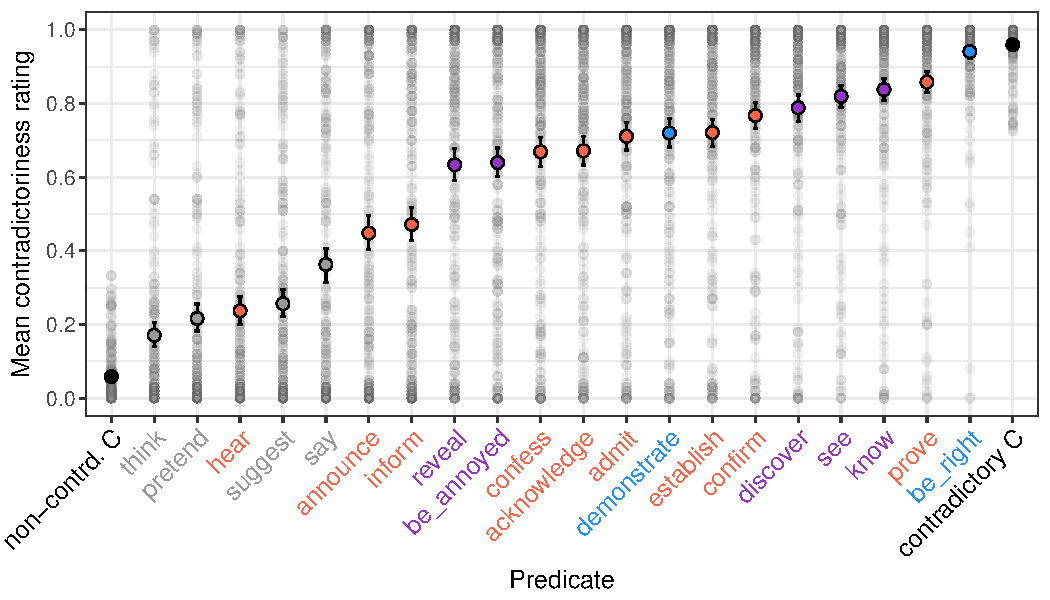
\includegraphics[width=.7\paperwidth]{../results/2-veridicality2/graphs/means-contradictoriness-by-predicate-variability}

\caption{Mean contradictoriness rating by predicate, collapsing over complements, including the non-contradictory controls (`non-contrd.\ C') and the contradictory controls (`contradictory C'). Error bars indicate 95\% confidence intervals. Light gray dots indicate individual participants' ratings. Factive predicates are given in violet, veridical non-factive ones in blue, projective non-factive ones in orange and plain non-factive ones in gray.}
\label{f-veridicality-predicate2}
\end{figure}

To determine which clause-embedding predicates are such that the content of the complement is entailed, i.e., for which clause-embedding predicates the strength of the inference to the content of the complement is at ceiling, we fit a Bayesian model predicting rating from predicate. Random effects for item and participant. SLOPE? 

Results: which ones are indistinguishable from entailing controls?


%\begin{table}[h!]
%\setlength\tabcolsep{3pt}
%
%\centering
%\small
%
%\begin{tabular}{l l l l l l l l l l l l l l l l l l l l l}
%\toprule
%
% &   \rot{\color{brown}{\em think}\color{black}} & \rot{\color{brown}{\em pretend}\color{black}} & \rot{\color{black}{\em hear}\color{black}} &  \rot{\color{brown}{\em suggest}\color{black}} &  \rot{\color{brown}{\em say}\color{black}} & \rot{{\em announce}} & \rot{{\em inform}} & \rot{\color{blue}{\em reveal}\color{black}} & \rot{\color{blue}{\em be annoyed}\color{black}} & \rot{{\em acknowledge}} & \rot{{\em confess}} & \rot{{\em admit}} & \rot{\color{airforceblue}{\em demonstrate}\color{black}}  & \rot{\color{black}{\em establish}}  & \rot{{\em confirm}}  & \rot{\color{blue}{\em discover}\color{black}} & \rot{\color{blue}{\em see}\color{black}}  & \rot{\color{blue}{\em know}\color{black}}  & \rot{{\em prove}} & \rot{\color{airforceblue}{\em be right}\color{black}} \\
%\midrule
%%\color{brown}{\em think}\color{black}		& x & - & - & - & - & - & - & - & - & - & - & - & - & - & - & - & - & - & - \\
%\color{brown}{\em pretend}\color{black}		& n.s. & - & - & - & - & - & - & - & - & - & - & - & - & - & - & - & - & - & - & - \\
%\color{black}{\em hear}\color{black}			& n.s. & n.s. & - & - & - & - & - & - & - & - & - & - & - & - & - & - & - & - & - & -\\
%\color{brown}{\em suggest}	\color{black}		& * & n.s. & n.s. & - & - & - & - & - & - & - & - & - & - & - & - & - & - & - & - & -\\
%\color{brown}{\em say}\color{black}		& *** & *** & *** & ** & - & - & - & - & - & - & - & - & - & - & - & - & - & - & - & -\\
%\color{black}{\em announce}\color{black}		& *** & *** & *** & *** & * & - & - & - & - & - & - & - & - & - & - & - & - & - & - & -\\
%\color{black}{\em inform}\color{black}		& *** & *** & *** & *** & ** & n.s. & - & - & - & - & - & - & - & - & - & - & - & - & - & -\\
%\color{blue}{\em reveal}\color{black}		& *** & *** & *** & *** & *** & *** & *** & - & - & - & - & - & - & - & - & - & - & - & - & -\\
%\color{blue}{\em be annoyed}\color{black}		& *** & *** & *** & *** & *** & *** & *** & n.s. & - & - & - & - & - & - & - & - & - & - & - & -\\
%\color{black}{\em acknowledge}\color{black}		& *** & *** & *** & *** & *** & *** & *** & n.s. & n.s. & - & - & - & - & - & - & - & - & - & - & -\\
%\color{black}{\em confess}\color{black}	& *** & *** & *** & *** & *** & *** & *** & n.s. & n.s. & n.s. & - & - & - & - & - & - & - & - & - & -\\
%\color{black}{\em admit}\color{black}			& *** & *** & *** & *** & *** & *** & *** & * & . & n.s. & n.s. & - & - & - & - & - & - & - & - & -\\
%\color{airforceblue}{\em demonstrate}\color{black}		& *** & *** & *** & *** & *** & *** & *** & ** & * & n.s. & n.s. &  n.s. & - & - & - & - & - & - & - & -\\
%\color{black}{\em establish}\color{black}	& *** & *** & *** & *** & *** & *** & *** & ** & * & n.s. & n.s. & n.s. & n.s. & - & - & - & - & - & - & -\\
%\color{black}{\em confirm}\color{black}		& *** & *** & *** & *** & *** & *** & *** & *** & *** & ** & ** & n.s. & n.s. & n.s. & - & - & - & - & - & -\\
%\color{blue}{\em discover}\color{black}		& *** & *** & *** & *** & *** & *** & *** & *** & *** & *** & *** & n.s. & n.s. & n.s. & n.s. & - & - & - & - & -\\
%\color{blue}{\em see}\color{black}			& *** & *** & *** & *** & *** & *** & *** & *** & *** & *** & *** & ** & ** & ** & n.s. & n.s. & - & - & - & -\\
%\color{blue}{\em know}\color{black}			& *** & *** & *** & *** & *** & *** & *** & *** & *** & *** & *** & *** & *** & *** & n.s. & n.s. & n.s. & - & - & -\\
%\color{black}{\em prove}\color{black}			& *** & *** & *** & *** & *** & *** & *** & *** & *** & *** & *** & *** & *** & *** & ** & . & n.s. & n.s. & -  & -\\
%\color{airforceblue}{\em be right}\color{black}		& *** & *** & *** & *** & *** & *** & *** & *** & ***  & ***  & *** & *** & *** & *** & *** & *** & *** & ** & *  & -\\
%\color{black}controls (\ref{control-bad})\color{black}		& *** & *** & *** & *** & *** & *** & *** & *** & ***  & ***  & *** & *** & *** & *** & *** & *** & *** & *** & ***  & n.s. \\
%
%\bottomrule
%\end{tabular}
%\caption{P-values associated with pairwise comparison of contradictoriness ratings of clause-embedding predicates and the controls in (\ref{control-bad}) using Tukey's method. `***' indicates significance at .0001, `**' at .01, `*' at .05, `.' marginal significance at .1, and `ns' indicates no significant difference in means. factive predicates are given in darker blue, veridical non-factive ones in lighter blue, plain non-factive ones in brown and projective non-factive ones in black.}\label{t-pairwise}
%\end{table}

\subsection{Discussion}\label{s33}

In Experiments 2 we applied two standard diagnostics for entailment to the contents of the complements of 20 clause-embedding predicates with the goal of identifying whether the contents are entailed. Given the definition of entailment, we assumed that if the content of the complement of a predicate is entailed, responses under either diagnostic are at ceiling, i.e., statistically indistinguishable from the relevant controls; otherwise, the content is not entailed.\footnote{One can, of course, imagine other linking functions for the two entailment experiments. For instance, one could assume a linking function according to which the content of the complement of a predicate is entailed if and only if the mean response to stimuli with the predicate is above .8. However, such a linking function is incompatible with the definition of entailment according to which the content of $\phi$ does not entail the content of $\psi$ if there is one world in which the content of $\phi$ is true and the content of $\psi$ is false. Furthermore, it is unclear how a non-arbitrary threshold could be chosen: why .8 rather than .85 or .75? And, finally, such a linking function would still not support the standard assumption that the content of the complement of factive and veridical non-factive predicates is entailed and that of plain non-factive and projective non-factive predicates is not: with a threshold of .8 on Exp.~2b, for instance, the content of the complement of the factive predicates {\em reveal, discover} and {\em be annoyed} and of the veridical non-factive predicate {\em demonstrate} would not be considered to be entailed, but that of the projective non-factive predicate {\em prove} would be.} Table \ref{t-summary} summarizes the findings of the two experiments: `$\checkmark$' indicates that the strength of the inference to the content of the complement (Exp.~2a) or the contradictoriness rating (Exp.~2b) was at ceiling; `$\times$' indicates that the strength of the inference or the contradictoriness rating was significantly lower than ceiling. As shown, the veridical non-factive predicate {\em be right} is the only predicate for which the responses were at ceiling in both experiments. For the factive predicates {\em see, discover, know} and {\em be annoyed}, and for the projective non-factive predicates {\em prove} and {\em confirm}, the responses in Exp.~2b were significantly lower than ceiling. For all other predicates, responses in both experiments were significantly lower than ceiling


\begin{table}[h!]
%\setlength\tabcolsep{3pt}

\centering
\small

\begin{tabular}{r c c c c c c c c c c c c c c c c c c c c}

Exp.\ & \rot{\color{airforceblue}{\em be right}\color{black}} &  \rot{\color{blue}{\em see}\color{black}} & \rot{\color{blue}{\em discover}\color{black}} & \rot{\color{blue}{\em know}\color{black}} & \rot{\color{blue}{\em be annoyed}\color{black}} & \rot{\color{black}{\em prove}\color{black}} & \rot{\color{black}{\em confirm}\color{black}} & \rot{\color{black}{\em establish}\color{black}} & \rot{\color{black}{\em admit}\color{black}} & \rot{\color{black}{\em acknowledge}\color{black}} & \rot{\color{airforceblue}{\em demonstrate}\color{black}} &  \rot{\color{blue}{\em reveal}\color{black}} & \rot{\color{black}{\em hear}\color{black}} & \rot{\color{black}{\em confess}\color{black}} & \rot{\color{black}{\em inform}\color{black}} & \rot{\color{black}{\em announce}\color{black}} & \rot{\color{brown}{\em say}\color{black}} & \rot{\color{brown}{\em suggest} \color{black}} & \rot{\color{brown}{\em pretend}\color{black}} & \rot{\color{brown}{\em think}\color{black}} \\ 

\toprule

2a & $\checkmark$ & $\checkmark$& $\checkmark$& $\checkmark$& $\checkmark$& $\checkmark$& $\checkmark$ & $\times$ & $\times$ &  $\times$ & $\times$ & $\times$ & $\times$ & $\times$ & $\times$ & $\times$ & $\times$ & $\times$ & $\times$ & $\times$ \\

2b & $\checkmark$ & $\times$ & $\times$ &  $\times$ & $\times$ & $\times$ & $\times$ & $\times$ & $\times$ & $\times$ & $\times$ & $\times$ & $\times$ & $\times$ & $\times$ & $\times$ & $\times$ & $\times$ & $\times$ & $\times$\\

\bottomrule
\end{tabular}
\caption{Findings of Exps.~2a and 2b for the 20 clause-embedding predicates. factive predicates are given in darker blue, veridical non-factive ones in lighter blue, plain non-factive ones in brown and projective non-factive ones in black. `$\checkmark$' indicates that responses were at ceiling;  `$\times$' indicates that responses were significantly lower than ceiling.}\label{t-summary}
\end{table}

For 14 of the 20 clause-embedding predicates, the findings of the two experiments converge. First, the findings of both experiments support an analysis of the content of the complement of the veridical non-factive predicate {\em be right} as entailed because responses in both experiments to stimuli with this predicates were at ceiling. Second, the findings of both experiments support an analysis of 13 predicates as not entailed because responses in both experiments to stimuli with these predicates were lower than ceiling:  these 13 predicates include the plain non-factive predicates {\em say, suggest, pretend} and {\em think}, the projective non-factive predicates {\em establish, admit, acknowledge, hear, confess, inform} and {\em announce}, but also the purportedly factive predicate {\em reveal} and the purportedly veridical non-factive predicate {\em demonstrate}. Thus, for {\em reveal} and {\em demonstrate}, the findings do not support the prevailing assumption that the content of the complement of these predicates is entailed. 

For the remaining 6 clause-embedding predicates, the findings of the two experiments differ: for the factive predicates  {\em see, discover, know} and {\em be annoyed}  and the projective non-factive predicates {\em prove} and {\em confirm}, the inference to the content of the complement was at ceiling in Exp.~2a, supporting an analysis of the content of the complement as entailed, but the contradictoriness ratings were below ceiling in Exp.~2b, supporting an analysis as not entailed. Thus, for these 6 factive and projective non-factive predicates, the findings of the entailment experiments are weaker but nevertheless critical with respect to the question of which clause-embedding predicates are such that the content of their complement is entailed: the experiments do not support the standard assumption that the contents of some of these predicates are entailed and others are not entailed. Rather, these 6 predicates are indistinguishable under the two entailment diagnostics.

This finding also bears on the debate that was introduced in section \ref{s1}, about whether the content of the complement of the emotive predicate {\em be annoyed} and the cognitive predicate {\em know} is entailed. Some authors, like \citet{klein1975,giannakidou1998,schlenker2003} and \citet{egre2008}, took examples like (\ref{emotive2}a) and (\ref{fis}b), repeated below for convenience, to show that the content is not entailed. Other authors, like \citet{gazdar79a} and \citet{abrusan2011}, did not take such examples to counter-exemplify an analysis of the content of the complement as entailed. These authors instead suggested that such examples are cases of free indirect discourse or are understood with a different concept of knowledge. Under this proposal, (\ref{emotive2}a), for instance, ``reports an attitude of a subject towards facts as perceived by him'' (\citealt[514]{abrusan2011}). As a consequence, ``the implications of [(\ref{emotive2}a)] do not have to be shared by the speaker''  ({\em ibid.}), which accounts for the observation that the content of the complement does not follow from (\ref{emotive2}a). Similarly, \citet[515]{abrusan2011} suggested that speakers or writers of examples like (\ref{fis}b) ``are understood as reporting a belief or feeling of ``knowledge'' on somebody's part'', but not necessarily on part of the speaker. 

\begin{exe}

\exi{(\ref{emotive2}a)} Falsely believing that he had inflicted a fatal wound, Oedipus regretted killing the stranger on the road to Thebes \hfill (\citealt{klein1975})

\exi{(\ref{fis}b)} Everyone knew that stress caused ulcers, before two Australian doctors in the early 80s proved that ulcers are actually caused by bacterial infection. \hfill (\citealt[501]{hazlett2010})

\end{exe}
The findings of our experiments replicate the two positions of the debate. On the one hand, the findings of Exp.~2a show that the strength of the inference to the truth of the content of the complement of {\em be annoyed} and {\em know} is at ceiling. On the other hand, the findings of Exp.~2b show that speakers who utter sentences with such predicates need not be (taken to be) committed to the truth of the content of the complement. Advocates of the position that the content of the complement of {\em be annoyed} and {\em know} is entailed might argue that the findings of Exp.~2b do not counter-exemplify the analysis of the content as entailed because the speakers in Exp.~2b were presented as not being committed to the truth of the content of the complement (e.g., Christopher: {\em ``Melissa knows/is annoyed that Danny ate the last cupcake, but he didn't.''}). This, in turn, may have resulted in participants understanding these utterances as ``reporting a belief or feeling of knowledge'' on the attitude holder's part. We agree that this is a possible interpretation and, therefore, the findings of our entailment experiments do not resolve the question of whether the content of the complement of {\em be annoyed} and {\em know} is entailed. Importantly, however, this interpretation would apply not only to the factive predicates we investigated in Exp.~2b, but also to the non-factive predicates {\em prove} and {\em confirm}, which patterned like the factive predicates {\em see, discover, know} and {\em be annoyed} on both entailment experiments. Thus, this interpretation would not support the standard distinction between the purportedly factive predicates {\em see, discover, know} and {\em be annoyed}, on the one hand, and the purportedly non-factive ones  {\em prove} and {\em confirm}, on the other.

The two entailment diagnostics gave different results for the contents of the complements of the 20 clause-embedding predicates. Specifically, we  observe that there were more lower-than-ceiling responses under the contradictoriness diagnostics in Exp.~2b than under the inference diagnostic in Exp.~2a. As a consequence, the findings of Exp.~2a support an analysis of the content of the complement as  entailed for more predicates than the findings of Exp.~2b. We hypothesize that this difference is due to a difference in task demand. In order to give a not-at-ceiling response under the inference diagnostic, participants had to imagine a world in which the statement that was presented as true (e.g., {\em Mark informed Sam / established that Sophie got a tattoo}) is true and in which the content of the complement (e.g., {\em Sophie got a tattoo}) is false. Evidence that this task is challenging comes from the observation that even trained researchers can fail to imagine such a world (see section \ref{s1}). By contrast, to give a not-at-ceiling response under the contradictoriness diagnostic, participants merely had to assess the speaker's utterance as not entirely contradictory. 

Does the observation that the two entailment diagnostics give different results mean that one of them is more suitable to diagnosing entailment?  Entailment is a semantic notion, and the two diagnostics differ in whether they force participants to consider contextual information. Specifically, on the contradictoriness diagnostic, participants must consider utterances by a speaker and the consistency of the epistemic state of this speaker, whereas, on the inference diagnostic, they consider true statements, not utterances, and no other epistemic agent. One might therefore be tempted to assume that the inference diagnostic is more suitable to diagnosing the semantic notion of entailment. However, in view of the aforementioned task demand of the inference diagnostic, it may be that the inference diagnostic may result in false positives (i.e., affirms an entailment relationship where there isn't one) whereas the contradictoriness diagnostic may result in false negatives (i.e., denies an entailment relationship where there is one). Furthermore, as discussed in \citealt{demarneffe-etal2012}, even judgments about what follows from utterances may be influenced by pragmatic information. For instance, the presumed trustworthiness of the attitude holder may influence not just contradictoriness ratings but also inference ratings.

Resolving the question of how to best diagnose entailment with theoretically untrained speakers is not possible in the scope of this paper. We note, however, that resolving this question is of central importance for research that makes use of the notion of entailment in the analysis of the meanings of sentences with clause-embedding predicates, like projection analyses, as we discuss in the next section.

\section{Discussion}\label{s4}

The experiments reported on in the previous two sections were designed to investigate whether the contents of the complements of 20 English clause-embedding predicates are projective (Exp.~1) and entailed (Exps.~2), with the goal of identifying whether the long-standing and widely-assumed categorical division between factive and non-factive predicates is empirically supported. Specifically, our experiments investigated projectivity and entailment for 5 factive predicates, namely {\em be annoyed, know, see, discover} and {\em reveal}, as well as for 15 non-factive predicates, namely the plain non-factive predicates {\em pretend, suggest, say} and {\em think}, the veridical non-factive predicates {\em be right} and {\em demonstrate}, and the projective non-factive predicates {\em acknowledge, admit, announce, confess, confirm, establish, hear, inform} and {\em prove}. Given the prevailing classifications of these predicates, we expected the contents of their complements to pattern alike with respect to projectivity and entailment. However, our experiments identified significant within-class variation in both projectivity and entailment:

\begin{itemize}[topsep=-1pt,itemsep=1pt]

\item {\bf factive predicates:} The content of the complement of these predicates is expected to be projective and entailed. There is, however, no empirical support for the assumption that the content of the complement of {\em reveal} is entailed, and only partial support for the remaining 4 predicates. Furthermore, there is by-predicate projection variability.

\item {\bf plain non-factive predicates:} The content of the complement of these predicates is expected to be neither projective nor entailed. However, only the content of the complement of {\em pretend} is not projective; that of the other 3 predicates is at least weakly projective.

\item {\bf veridical non-factive predicates:} The content of the complement of these predicates is expected to be entailed but not projective. Contrary to expectation, the content of the complement of both predicates investigated is at least weakly projective, and there is no empirical support for the assumption that the content of the complement of {\em demonstrate} is entailed. 

\item {\bf projective non-factive predicates:} The content of the complement of these predicates is expected to be projective but not entailed. However, for {\em prove} and {\em confirm}, there is support for an analysis of the content of the complement as entailed. Furthermore, there is by-predicate projection variability.

\end{itemize}

In sum, our experiments did not find empirical support for the assumption that the content of the complement of predicates in each of these four classes patterns alike. With respect to entailment, there is only partial support for many of the factive and veridical non-factive predicates that the content of the complement is entailed; for {\em reveal} and {\em demonstrate} there is no support at all, and hence these predicates cannot be assumed to be factive and veridical non-factive, respectively. Furthermore, the experiments identified significant with-class projection variability, which calls into question the naturalness of these four classes of predicates. 

Do the experiments support a different classification of the 20 predicates under investigation into factive and (various types of) non-factive ones? To answer this question, consider Figure \ref{f-summary-categorical}, which plots the mean certainty rating of the contents of the complements in Exp.~1 on the x-axis and, on the y-axis, whether the content of their complement is entailed under, in the left panel (a), the inference diagnostic of Exp.~2a and, in the right panel (b), the contradictoriness diagnostic of Exp.~2b. 

\begin{figure}[h]

\begin{subfigure}{.5\textwidth}
\centering
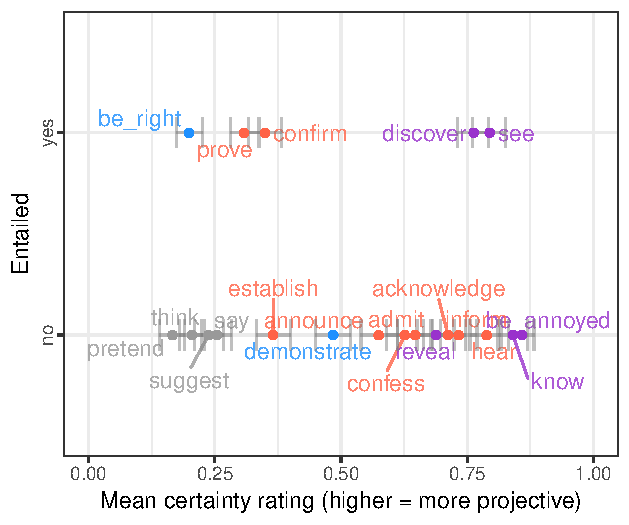
\includegraphics[width=.35\paperwidth]{../results/5-projectivity-no-fact/graphs/projection-by-inferenceEntailment}
\caption{Inference diagnostic for entailment}
\end{subfigure}%
\begin{subfigure}{.5\textwidth}
\centering
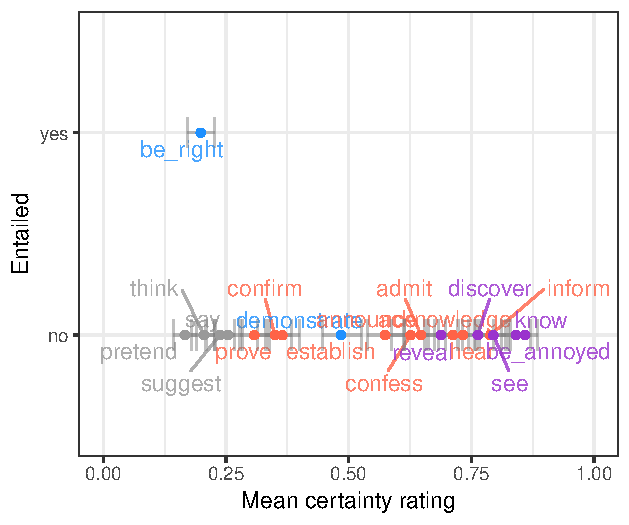
\includegraphics[width=.35\paperwidth]{../results/5-projectivity-no-fact/graphs/projection-by-contradictorinessEntailment}
\caption{Contradictoriness diagnostic for entailment}
\end{subfigure}

\caption{Properties of the contents of the complements of 20 English clause-embedding predicates: on the x-axis, the mean certainty rating (with 95\% confidence intervals) and, on the y-axis, whether the content of the clausal complement is entailed under (a) the inference diagnostic of Exp.~2a or (b) the contradictoriness diagnostic of Exp.~2b. factive predicates are given in darker blue, veridical non-factive ones in lighter blue, plain non-factive ones in brown and projective non-factive ones in black.}\label{f-summary-categorical}

\end{figure}

Does a class of factive predicates emerge from the experiments? Given the findings of the inference diagnostic for entailment (left panel of Figure \ref{f-summary-categorical}), there are four predicates for which the content of the clausal complement is both entailed and relatively highly projective, namely {\em discover, be annoyed, see} and {\em know}. Whether a predicate like {\em confirm, prove} or {\em be right} should count as factive depends on how projective the content of the complement needs to be in order for the predicate to be considered factive: the contents of the complements of {\em confirm, prove} or {\em be right} are significantly less projective than that of {\em discover, be annoyed, see} and {\em know}, but that of {\em discover} is also significantly less projective than that of {\em know} and {\em be annoyed}. It is unclear where a non-arbitrary line could be drawn between predicates, given that the contents of the complements of {\em confirm, prove} and {\em be right} are not non-projective, just less projective. Furthermore, no class of factive predicates appears to emerge given the findings of the  contradictoriness diagnostic for entailment (right panel). In short, our experiments do not provide clear empirical support for a class of factive predicates: whether there is such a class depends on how entailment is best diagnosed and how projective the content of the complement of a clause-embedding predicate needs to be to count as factive.

Given the finding that the content of the complement of {\em pretend} is not projective, the experiments can be taken to support a class of plain non-factive predicates for which the content of the complement is neither entailed nor projective. Which other predicates belong to this class is an open question. There is also empirical support for a class of projective non-factive predicates, i.e., predicates for which the content of the complement is projective but not entailed. In fact, this class appears to be quite large, given that the content of the complement of many more predicates than previously assumed is at least weakly projective. Of course, which predicates are projective non-factive ones again depends on the question of how entailment is best diagnosed. Furthermore, this class would be quite heterogeneous, given the rampant by-predicate projection variability, which again calls into question the naturalness of such a class of predicates. Finally, our experiments do not provide support for a class of veridical non-factive predicates, i.e., predicates for which the content of the complement is entailed but not projective. For instance, the content of the complement of {\em be right} is entailed but also weakly projective, and the content of the complement of {\em pretend} is not projective (as noted above) but also not entailed. 

In sum, the experiments provide straightforward support neither for the standard classification of the 20 clause-embedding predicates into factive and (various types of) non-factive ones nor for an alternative classification. The main issues with supporting such a categorical classification are that it is not clear i) how entailment is best diagnosed and ii) how gradient projectivity can motivate a binary classification. 

Resolving these issues is of critical importance for research that builds on the distinction between factive and non-factive predicates, like formal analyses of projection, as introduced in section \ref{s1}. Both lexicalist analyses (e.g., \citealt{heim83,vds92}) and entailment-based analyses (e.g., \citealt{abrusan2011,abrusan2016,romoli2015,best-question}) are challenged by our findings. Lexicalist analyses, on which the content of the complement of factive predicates is lexically specified as a presupposition, must resolve which clause-embedding predicates are factive; entailment-based analyses, on which the projectivity of the content of the complement is derived from its status as entailed content, must resolve for which clause-embedding predicates the content of the complement is entailed. Furthermore, entailment-based analyses also need to confront the observation that there may be contents that are entailed but only weakly projective. For instance, given the findings of the inference diagnostic for entailment (see panel (a) of Figure \ref{f-summary-categorical}), the content of the complement of {\em be right} and {\em confirm} is entailed but only weakly  ({\em be right}) or mildly ({\em confirm}) projective. On Abrus\'an's (2011, 2016) analysis, entailed content is predicted to not project if projection is incompatible with the asserted content or an implicature of the assertion, or if the content addresses the grammatically signaled background question (\citealt[511, 532]{abrusan2011}). On  \citetpos{best-question} analysis, entailed content is predicted to not project if the content is not entailed by the Question Under Discussion. Whether these analyses can systematically account for entailed content that is less projective is a question for future research (see also \citealt{tbd-variability} on this point).

The findings of Exp.~1 also show that the empirical purview of projection analyses is broader than previously assumed, given that the contents of the complements of almost all of the 20 clause-embedding predicates emerged as projective, albeit to varying degrees. To date, there are only very few formal analyses of the projectivity of the content of the complement of non-factive predicates.  One attempt is presented in \citealt{schlenker10}, who proposed that {\em announce} is a ``part-time presupposition trigger'' (p.139): ``in some contexts, [{\em announce}, JT\&JD] does not entail the truth of its complement; in other contexts, it entails and {\em presupposes} the truth of the complement'' ({\em ibid.}). The notion of entailment adopted by Schlenker appears to be a context-dependent one, not the standard notion assumed here. We refer to his notion as `Schlenker-entailment': in context $c$, the content of sentence $\phi$ Schlenker-entails the content of sentence $\psi$ if and only the truth of $\psi$ follows from the truth of $\phi$ in $c$.  Thus, on Schlenker's proposal, a context in which the content of the complement of {\em announce} projects is a context in which a true assertion of the unembedded sentence with {\em announce} Schlenker-entails the content. Abstracting over contexts, it follows that if the content of the complement of {\em announce} is less projective than that of some other clause-embedding predicate $P$, we expect the content of the complement of {\em announce} to follow less strongly from true assertions of unembedded sentences with {\em announce} than from such assertions with $P$. This expectation is not borne out: the content of the complement of {\em announce} is less projective than that of {\em hear} (Exp.~1), but on both the inference diagnostic (Exp.~2a) and the contradictoriness diagnostic (Exp.~2b), the content of the complement of {\em announce} received significantly higher responses than that of {\em hear}. We conclude that the findings of our experiments are not predicted by \citetpos{schlenker10} proposal for the projectivity of the content of the complement of non-factive predicates like {\em announce}.

Another proposal to derive projectivity for non-factive predicates is presented by \citet{spector-egre2015}, who proposed (p.1736) that predicates like {\em tell, predict} and {\em announce}  are ambiguous between a factive lexical entry on which the content of the complement is entailed and presupposed, and thereby projective, and a non-factive one on which it is not. One concern with this proposal is that it is not clear where to draw lines between predicates: which predicates only have a factive lexical entry, which ones have both a factive and a non-factive one, which ones have only have a non-factive one? Given our finding that {\em pretend} is the only one of the 20 clause-embedding predicates explored for which the content of the complement is not projective, a second concern with this proposal is that it may require the assumption of widespread ambiguity among clause-embedding predicates. Finally, it is not clear whether the proposal can account for the observed by-predicate projection variability. For instance, the assumption that {\em discover} and {\em be annoyed} only have a factive lexical entry does not suffice to predict that the content of the complement of {\em discover} is less projective than that of {\em be annoyed}; likewise, the assumption that {\em inform} and {\em announce} have both a factive and a non-factive lexical entry does not suffice to predict that the content of the complement of {\em announce} is less projective than that of {\em inform}.

A third proposal is sketched by \citet{anand-hacquard2014}: these authors suggested that speakers may be taken to be committed to the content of the complement of so-called assertive predicates like {\em acknowledge, admit} and {\em confirm} ``because of the kind of discourse moves that these predicates report'' (p.74). Specifically, utterances of sentences with these predicates can be used to report the success of an uptake in a reported common ground: for example, an utterance of a sentence like {\em Kim confirmed that Mary is the murderer} can report that the content $p$ of the  complement, that Mary is the murderer, is accepted ``into the common ground of the reported discourse'' ({\em ibid.}). The authors suggested that ``[t]his acceptance of $p$ can easily bleed into the actual common ground, under the assumption that no subsequent move removed $p$ from the common ground'' (p.74f). The authors briefly entertained an extension of this proposal to utterances of sentences with {\em inform} and {\em announce}, which convey that the content of the complement is part of the reported common ground: ``to the extent that we identify ourselves with that context'' (p.76), the speaker and the addressee are committed to the truth of the content of the complement. While this proposal would need to be fleshed out in more detail to be predictive, we are sympathetic to the idea that the discourse functions of utterances of sentences with clause-embedding predicates plays a role in deriving the projectivity of the content of the complement. The findings of Exp.~1 suggest, however, that more fine-grained distinctions between predicates and their discourse functions would need to be made because there are significant differences between predicates that \citet{anand-hacquard2014} suggested share discourse functions: the content of the complement of {\em confirm} is less projective than that of {\em admit} and {\em acknowledge}, and that of {\em announce} is less projective than that of {\em inform}. In sum, there is currently no projection analysis on the market that adequately accounts for the projectivity of the content of the complement of non-factive predicates. 

Where do we go from here? The two main findings of this paper are that i) projectivity and entailment, as diagnosed in this paper, do not straightforwardly support a categorical classification of predicates into factive and non-factive ones, and ii) the empirical purview of projection analyses is broader than previously assumed because the contents of the complements of many non-factive clause-embedding predicates are projective. These main findings motivate at least two fruitful ways forward, ways that are entirely compatible with one another. The first way forward is to identify whether other experimental implementations of the two standard entailment diagnostics or an application of a different entailment diagnostic altogether can provide better empirical support for the prevailing classification of predicates into ones for which the content of the complement is entailed and ones for which it is not. If such support can be provided, it is possible to continue to derive the projectivity of entailed content through a lexicalist or an entailment-based projection analysis (with the caveat, as discussed above and in \citealt{tbd-variability}, that current analyses do not predict the observed projection variability among factive predicates). 

The second way forward is to investigate how factors other than entailment are implicated in the projectivity of the content of the complement of clause-embedding predicates (and of other utterance content more generally). Factors that have already been identified in the literature as influencing the projectivity of utterance content are summarized in (\ref{factors}): 

\begin{exe}
\ex\label{factors} Factors influencing the projectivity of utterance content
\begin{xlist}

\ex Contextual information, including common ground (e.g., \citealt{gazdar79a,gazdar79b,tonhauser-etal-eval})

\ex Prior probability of events / lexical content (e.g., \citealt{tbd-variability})

\ex Lexical meaning and discourse function of the attitude predicate (e.g., \citealt{anand-hacquard2014,tbd-variability})

\ex Information structure, as marked for instance by prosody (e.g., \citealt{cummins-rohde2015,tonhauser-salt26,djaerv-bacovcin-salt27})

\ex At-issueness (e.g., \citealt{brst-salt10,best-question,abrusan2011,tbd-variability,mahler-nels})

\ex Perceived degree of reliability and trustworthiness of the attitude holder (e.g., \citealt{schlenker10,demarneffe-etal2012})

\end{xlist}
\end{exe}

As mentioned above, research on projectivity has been largely limited to entailed content. Many of the factors in (\ref{factors}), however, have already been shown to influence the projectivity of content regardless of whether it is entailed. \citet{tbd-variability}, for instance, investigated the projectivity of the content of the complement of many factive predicates, but also of {\em establish, confess} and {\em reveal} (having assumed that the content is entailed), and found that the factors prior probability, lexical meaning and at-issueness influence projectivity. Furthermore, as discussed above, \citet{anand-hacquard2014} assumed that the lexical meaning of a clause-embedding predicate influences the projectivity of the content of the complement of some non-factive predicates, and \citealt{schlenker10} and \citealt{demarneffe-etal2012} assumed that the trustworthiness of the attitude holder matters for non-factive predicates. These observations give rise to the following research questions: Which factors influence the projectivity of utterance content, including the contents of complements of clause-embedding predicates, and do they influence entailed and non-entailed content differently? Addressing these questions is an exciting avenue for future research and the answers to these questions hold the key to understanding whether distinct projection analyses are needed for entailed and non-entailed content.

\section{Conclusions}\label{s5}

This paper investigated the long-standing and widely-adopted distinction between factive and non-factive predicates on the basis of experiments designed to explore projectivity and entailment for the contents of the complements of 20 English clause-embedding predicates. These experiments revealed that i) projectivity and entailment do not straightforwardly support a categorical classification of predicates into factive and non-factive ones, and that ii) the empirical purview of projection analyses is broader than previously assumed. We also observed that current projection analyses do not adequately predict the projectivity of the contents of the complements of non-factive predicates, primarily because such analyses have limited their attention almost entirely to the contents of the complements of factive predicates. Our research thereby provides impetus for empirically-driven investigations of factors implicated in the projectivity of entailed as well as non-entailed content and the development of projection analyses for non-entailed content.


%Figure \ref{f-summary-gradient}: inference rating and contradictoriness ratings are also not good predictors
%
%\begin{figure}[h]
%\begin{subfigure}{.5\textwidth}
%\centering
%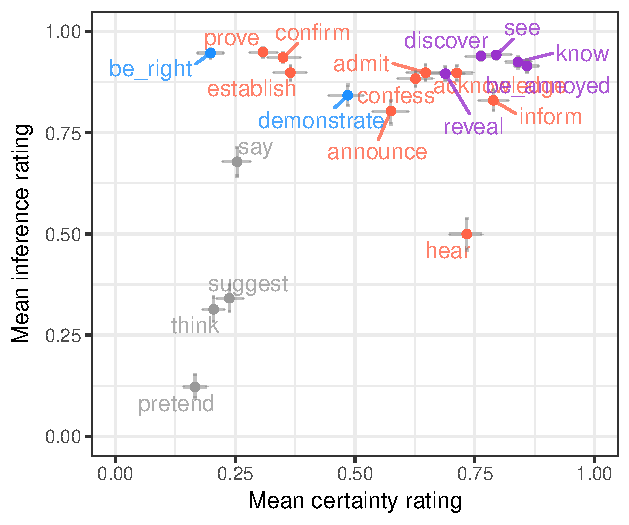
\includegraphics[width=.35\paperwidth]{../results/5-projectivity-no-fact/graphs/projection-by-inference}
%\caption{Inference diagnostic for entailment}
%\end{subfigure}%
%\begin{subfigure}{.5\textwidth}
%\centering
%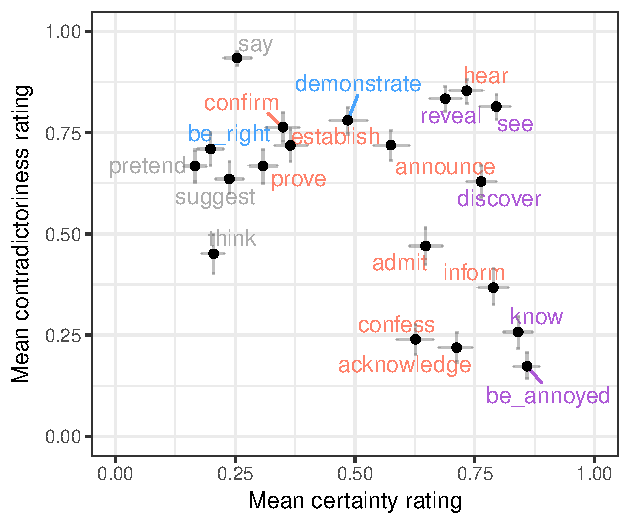
\includegraphics[width=.35\paperwidth]{../results/5-projectivity-no-fact/graphs/projection-by-contradictoriness}
%\caption{Contradictoriness diagnostic for entailment}
%\end{subfigure}
%\caption{Properties of the contents of the complements of 20 English clause-embedding predicates: on the x-axis, the mean certainty rating (with 95\% confidence intervals) and, on the y-axis, the mean inference rating from Exp.~2a (panel a) and the mean contradictoriness rating from Exp.~2b (panel b). factive predicates are given in darker blue, veridical non-factive ones in lighter blue, plain non-factive ones in brown and projective non-factive ones in black.}\label{f-summary-gradient}
%
%\end{figure}

\appendix

\setcounter{table}{0}
\renewcommand{\thetable}{A\arabic{table}}

\setcounter{figure}{0}
\renewcommand{\thefigure}{A\arabic{figure}}

%\section{Citations}
%
%That both properties are ascribed to presuppositions, including the content of the complement of factive predicates, can be seen from the following quotes:
%
%\begin{itemize}[topsep=0pt,itemsep=-3pt,leftmargin=12pt]
%
%\item \citealt[66f.]{beaver01}: \citet[119-123]{gazdar79a} ``describes the inferences associated with factive verbs, definite descriptions, aspectual verbs, and clefts as being indefeasible in simple affirmative sentences'', i.e., ``entailments''.
%
%\item \citealt[355]{ccmg90}: ``A sentence can both entail and presuppose another sentence [...]. Thus, [{\em Joan realizes that syntax deals with sentence structure}] both entails and presupposes [{\em Syntax deals with sentence struture}]."
%
%\item \citealt[345]{vds92}: ``Note that [global accommodation, i.e., projection, JT\&JD] is what we would expect given the intuitive notion of presupposition as information taken for granted and note also that this explains the intuition that presuppositions [...] are entailed by their matrix sentence.''
%
%\item \citealt[3]{abbott06}: ``we will need to be careful to distinguish entailments that are presupposed from what I will call ``ordinary, simple entailments'', which are not also presuppositions.''
%
%\item \citealt[139]{schlenker10}: ``we obtain the pattern of inference which is characteristic of presuppositions: an entailment of the positive sentence is preserved under negation and in questions''
%
%
%\item \citealt[77]{anand-hacquard2014}: ``we will adopt the pragmatic view of presupposition triggering, according to which presuppositions are lexical entailments that are backgrounded based on pragmatic principles"
%
%\item {\bf \citealt[fn.7]{spector-egre2015}: Assuming that any presupposition of a sentence is also an entailment of this sentence, it follows that a predicate that is factive with respect to its declarative complement is always also veridical with respect to its declarative complement.}
%
%\end{itemize}

\section{20 complement clauses}\label{a-clauses}

The following clauses realized the complements of the predicates in the three experiments: 

\begin{enumerate}[leftmargin=3ex,itemsep=-2pt]

\begin{multicols}{2}

\item Mary is pregnant.
\item Josie went on vacation to France.
\item Emma studied on Saturday morning.
\item Olivia sleeps until noon.
\item Sophia got a tattoo.
\item Mia drank 2 cocktails last night.
\item Isabella ate a steak on Sunday.
\item  Emily bought a car yesterday.
\item  Grace visited her sister.
\item Zoe calculated the tip.

\columnbreak

\item  Danny ate the last cupcake.
\item  Frank got a cat.
\item  Jackson ran 10 miles.
\item  Jayden rented a car.
\item  Tony had a drink last night.
\item  Josh learned to ride a bike yesterday.
\item  Owen shoveled snow last winter.
\item  Julian dances salsa.
\item  Jon walks to work.
\item  Charley speaks Spanish.

\end{multicols}

\end{enumerate}

\section{Experiments with binary response tasks}\label{a-clauses}

The three experiments reported on in this Appendix are identical to the three experiments in sections \ref{s2} and \ref{s3}, except that two-alternative forced choice ratings (`yes', `no') were collected rather than gradient ones. For each of the experiments, we recruited 600 participants with U.S.\ IP addresses and at least 99\% of previous HITs approved on Amazon's Mechanical Turk platform. They were paid \$1 for participating.

Prior to analysis, we excluded the data from participants who did not self-identify as native speakers of American English. If a participant took an experiment more than once, we only kept the data from the first time they took the experiment. We also excluded the data from participants who gave a wrong rating to at least one control: a rating was considered wrong if it was a `yes' rating on a projection control, a non-entailing control or a non-contradictory control, or a `no' rating on an entailing control or a contradictory control. The results presented below are based on data from 426 participants (ages 18-81; median: 37; 200 female, 220 male, 2 other) in the projection experiment, from 341 participants (ages 18- 73; median: 38; 180 female, 161 male) in the inference experiment and from 302 participants (ages 18-73; median: 37; 150 female, 152 male) in the contradictoriness experiment.

The findings of the experiments with the two-alternative forced choice task are shown in Figure \ref{f-binary}, which show the proportion of `yes' ratings by predicate, collapsing over complement clauses, in the projection experiment (panel a), in the entailment experiment with the inference diagnostic (panel b) and in the entailment experiment with the contradictoriness diagnostic (panel c). {\bf SAY SOMETHING ABOUT BMRS MODELS HERE}

\begin{figure}[H]
\centering

\begin{subfigure}{1\textwidth}
\centering
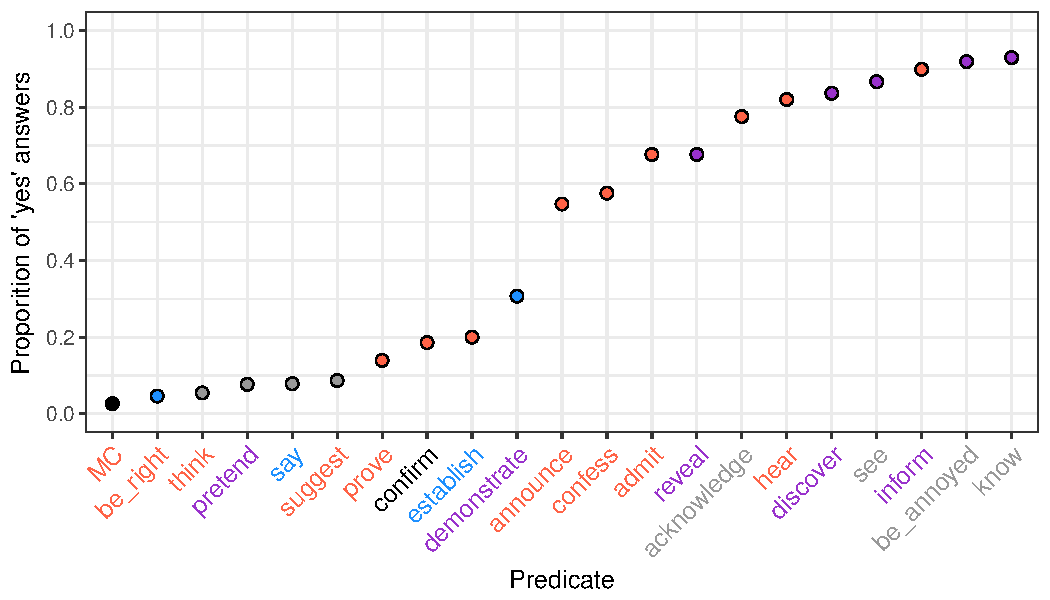
\includegraphics[width=.5\paperwidth]{../results/8-projectivity-no-fact-binary/graphs/proportion-by-predicate-variability}
\caption{`certain that' diagnostic for projection.}
\end{subfigure}

\begin{subfigure}{1\textwidth}
\centering
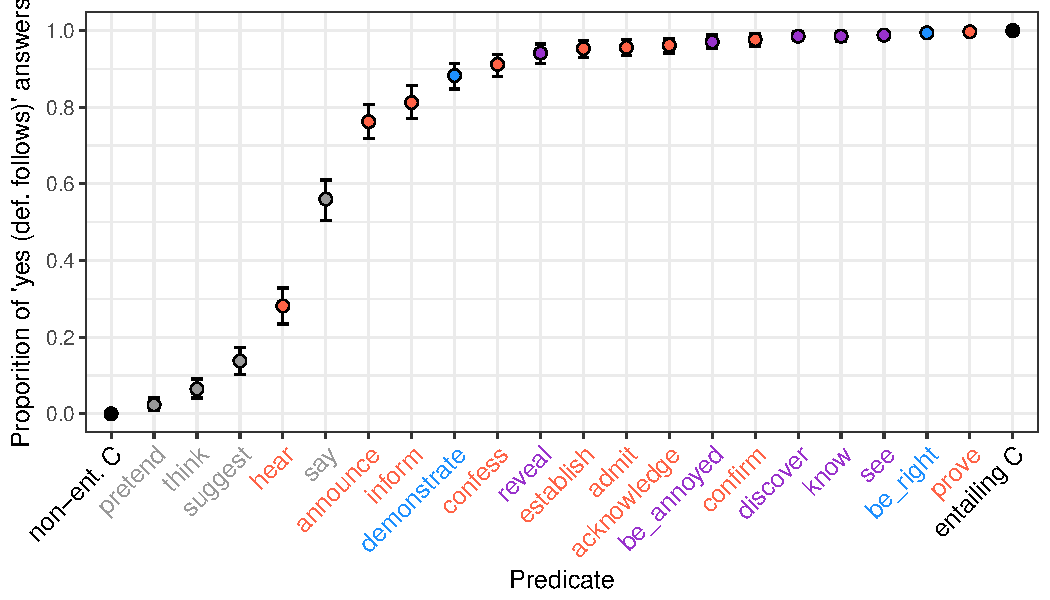
\includegraphics[width=.5\paperwidth]{../results/7-veridicality3-binary/graphs/proportion-by-predicate-variability}
\caption{Inference diagnostic for entailment. }
\end{subfigure}

\begin{subfigure}{1\textwidth}
\centering
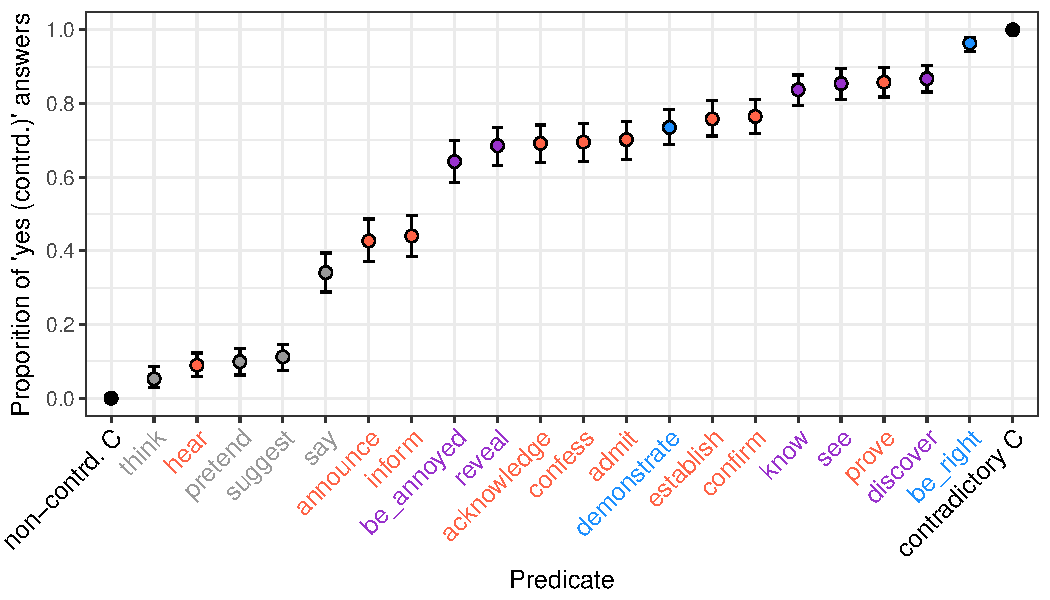
\includegraphics[width=.5\paperwidth]{../results/6-veridicality2-binary/graphs/proportion-by-predicate-variability}
\caption{Contradictoriness diagnostic for entailment}
\end{subfigure} 

\caption{Proportion of `yes' ratings with 95\% confidence intervals, collapsing over complement clauses. Controls are given in black, factive predicates in purple, veridical non-factive ones in blue, projective non-factive ones in orange and plain non-factive ones in gray.}
\label{f-binary}
\end{figure}

Figure \ref{f-comparison} allows for a comparison of the findings of the experiments with the gradient scales in sections \ref{s2} and \ref{s3} and the findings of the experiments with the two-alternative forced choice: these plots show the mean ratings on the gradient scales by the proportion of `yes' ratings in the two-alternative forced choice in the projection experiment (panel a), the entailment experiment with the inference diagnostic (panel b) and the entailment experiment with the contradictoriness diagnostic (panel c). Controls are given in black, factive predicates in purple, veridical non-factive ones in light blue, projective non-factive ones in orange and plain non-factive ones in gray. {\bf SAY SOMETHING ABOUT HOW SIMILAR FINDINGS ARE}
    
\begin{figure}[h!]
\centering

\begin{subfigure}{.33\textwidth}
\centering
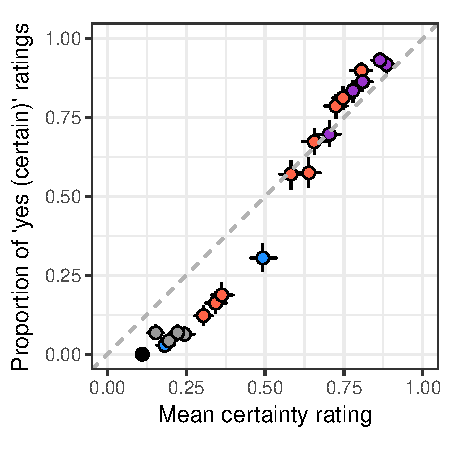
\includegraphics[width=.25\paperwidth]{../results/compare-binary-nonbinary/graphs/projectivity}
\caption{Projection}
\end{subfigure}~\quad    
\begin{subfigure}{.33\textwidth}
\centering
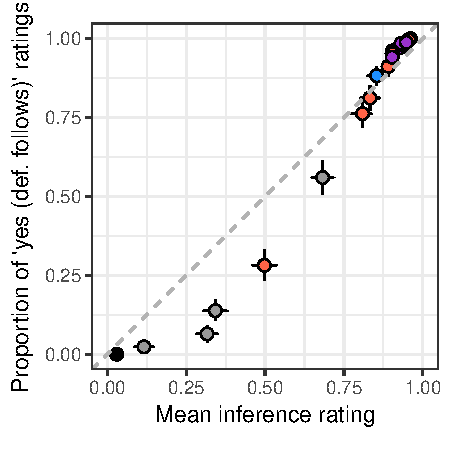
\includegraphics[width=.25\paperwidth]{../results/compare-binary-nonbinary/graphs/entailment-inference}
\caption{Inference}
\end{subfigure}~\quad   
\begin{subfigure}{.33\textwidth}
\centering
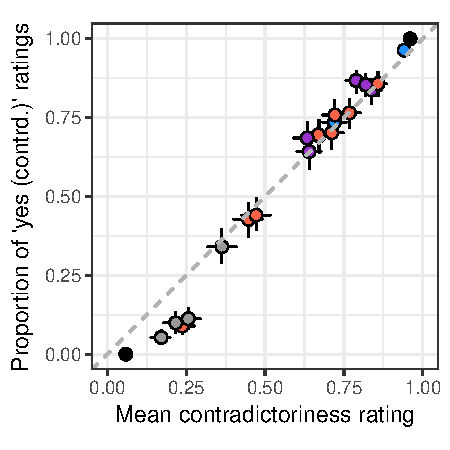
\includegraphics[width=.25\paperwidth]{../results/compare-binary-nonbinary/graphs/entailment-contradictory}
\caption{Contradiction}
\end{subfigure}    
   
\caption{Mean ratings on gradient scale by proportion of `yes' ratings in two-alternative forced choice, both with 95\% confidence intervals, collapsing over complement clauses. Controls are given in black, factive predicates in purple, veridical non-factive ones in light blue, projective non-factive ones in orange and plain non-factive ones in gray.}
\label{f-comparison}
\end{figure}


{\bf SPELL THIS OUT IN SUFFICIENT DETAIL FOR NON-EXPERIMENTAL PEOPLE:}

Spearman rank correlations (on target stimuli):

projection: 0.983

inference: 0.996

contradictoriness: 0.985

\bibliographystyle{/Users/tonhauser.1/Library/Latex/cslipubs-natbib}
\bibliography{/Users/tonhauser.1/Documents/bibliography}

\end{document}

